\documentclass{article}

\PassOptionsToPackage{table,svgnames}{xcolor}\usepackage{graphicx}
\usepackage{tikz-network}
\usepackage{xcolor}

\begin{document}
\begin{titlepage}
    \centering
    % Logo
    \includegraphics[width=0.6\textwidth]{logo-tec.png}\par\vspace{1cm}

    % University and course
    {\large Escuela de Ingeniería en Computación\par}
    {\large Investigación de Operaciones\par}
    \vspace{2cm}

    % Title
    {\Large Rutas Óptimas\par}
    {\large Algoritmo de Floyd\par}
    \vspace{2cm}

    % Group and professor
    {\large Grupo 40\par}
    {\large Profesor: Francisco Torres Rojas\par}
    \vspace{3cm}

    % Student info
    {\large Carmen Hidalgo Paz\par}
    {\large Carné: 2020030538\par}
    \vspace{1cm}
    {\large Melissa Carvajal Charpentier\par}
    {\large Carné: 2022197088\par}
    \vspace{1cm}
    {\large Josué Soto González\par}
    {\large Carné: 2023207915\par}
    \vspace{1cm}

    % Date
    {\large 12 de Septiembre del 2025\par}
\end{titlepage}
\definecolor{KirbyPink}{HTML}{D74894}
\definecolor{LightPink}{HTML}{FFBFBF}

\newpage


\section{Floyd's Algorithm}
This program consists of Floyd's algorithm to obtain the shortest path between any pair of nodes in a graph with weighted distances.
Floyd's algorithm compares the distance between any two given nodes and by passing through another city in between, if the result is less than the original then it chooses the shortest one. After contemplating all nodes in the graph, the graph is guaranteed to have all the shortest distances between any two nodes in the graph. These changes are recorded in another matrix called P that helps determine the shortest path between any two nodes.
\section{Robert W. Floyd (1936–2001)}
\begin{center}
\includegraphics[width=0.25\textwidth]{floyd.jpg}
\end{center}
Robert Willoughby Floyd was a computer scientist that lived from 1936 to 2001. He made great advances in computer science and developed an algorithm to find the shortest paths between any two nodes for a directed graph. He was awarded a Turing Award in 1978.


\section{Initial Graph}
\begin{center}
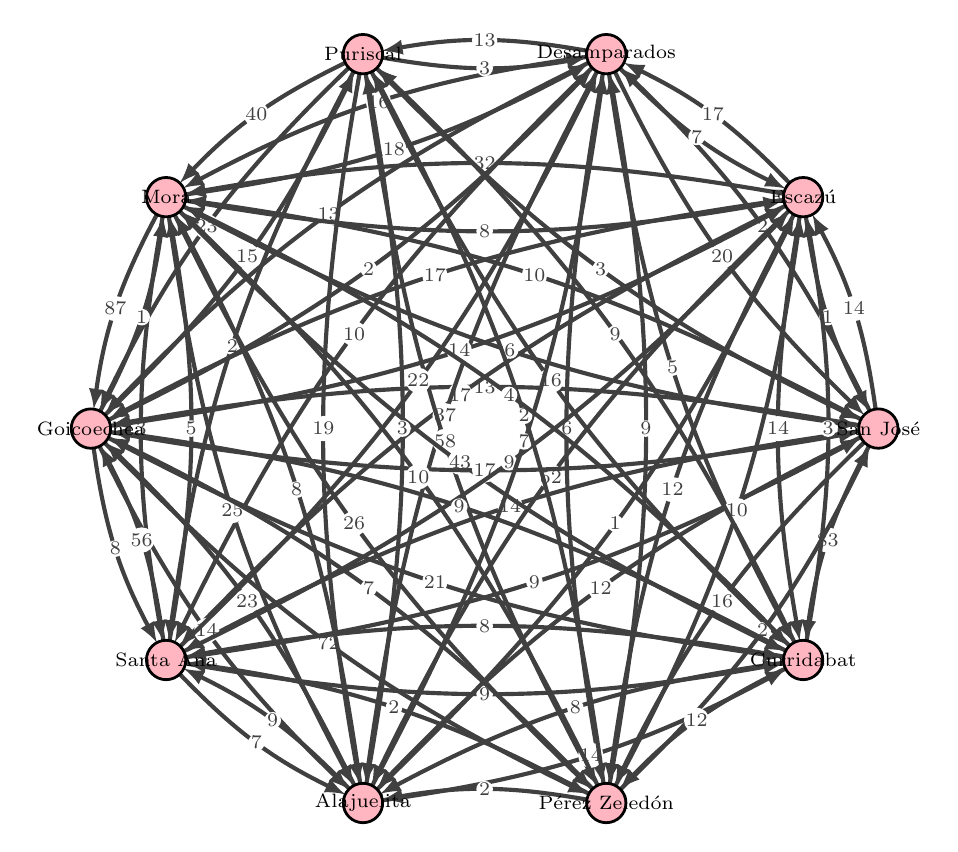
\begin{tikzpicture}
 \Vertex[x=5.000000, y=0.000000, color=LightPink, size=0.5, label={San José}]{A}
 \Vertex[x=4.045085, y=2.938926, color=LightPink, size=0.5, label={Escazú}]{B}
 \Vertex[x=1.545085, y=4.755282, color=LightPink, size=0.5, label={Desamparados}]{C}
 \Vertex[x=-1.545085, y=4.755282, color=LightPink, size=0.5, label={Puriscal}]{D}
 \Vertex[x=-4.045085, y=2.938926, color=LightPink, size=0.5, label={Mora}]{E}
 \Vertex[x=-5.000000, y=-0.000000, color=LightPink, size=0.5, label={Goicoechea}]{F}
 \Vertex[x=-4.045084, y=-2.938927, color=LightPink, size=0.5, label={Santa Ana}]{G}
 \Vertex[x=-1.545086, y=-4.755282, color=LightPink, size=0.5, label={Alajuelita}]{H}
 \Vertex[x=1.545086, y=-4.755282, color=LightPink, size=0.5, label={Pérez Zeledón}]{I}
 \Vertex[x=4.045086, y=-2.938925, color=LightPink, size=0.5, label={Curridabat}]{J}
 
 \Edge[bend=-10, label=$14$, Direct](A)(B) 
 \Edge[bend=-10, label=$2$, Direct](A)(C) 
 \Edge[bend=-10, label=$10$, Direct](A)(E) 
 \Edge[bend=-10, label=$13$, Direct](A)(F) 
 \Edge[bend=-10, label=$14$, Direct](A)(G) 
 \Edge[bend=-10, label=$12$, Direct](A)(H) 
 \Edge[bend=-10, label=$16$, Direct](A)(I) 
 \Edge[bend=-10, label=$83$, Direct](A)(J) 
 \Edge[bend=-10, label=$1$, Direct](B)(A) 
 \Edge[bend=-10, label=$17$, Direct](B)(C) 
 \Edge[bend=-10, label=$32$, Direct](B)(E) 
 \Edge[bend=-10, label=$17$, Direct](B)(F) 
 \Edge[bend=-10, label=$17$, Direct](B)(G) 
 \Edge[bend=-10, label=$52$, Direct](B)(H) 
 \Edge[bend=-10, label=$12$, Direct](B)(I) 
 \Edge[bend=-10, label=$14$, Direct](B)(J) 
 \Edge[bend=-10, label=$20$, Direct](C)(A) 
 \Edge[bend=-10, label=$7$, Direct](C)(B) 
 \Edge[bend=-10, label=$13$, Direct](C)(D) 
 \Edge[bend=-10, label=$16$, Direct](C)(E) 
 \Edge[bend=-10, label=$13$, Direct](C)(F) 
 \Edge[bend=-10, label=$10$, Direct](C)(G) 
 \Edge[bend=-10, label=$37$, Direct](C)(H) 
 \Edge[bend=-10, label=$6$, Direct](C)(I) 
 \Edge[bend=-10, label=$5$, Direct](C)(J) 
 \Edge[bend=-10, label=$3$, Direct](D)(A) 
 \Edge[bend=-10, label=$3$, Direct](D)(C) 
 \Edge[bend=-10, label=$40$, Direct](D)(E) 
 \Edge[bend=-10, label=$23$, Direct](D)(F) 
 \Edge[bend=-10, label=$2$, Direct](D)(G) 
 \Edge[bend=-10, label=$19$, Direct](D)(H) 
 \Edge[bend=-10, label=$58$, Direct](D)(I) 
 \Edge[bend=-10, label=$16$, Direct](D)(J) 
 \Edge[bend=-10, label=$6$, Direct](E)(A) 
 \Edge[bend=-10, label=$8$, Direct](E)(B) 
 \Edge[bend=-10, label=$18$, Direct](E)(C) 
 \Edge[bend=-10, label=$87$, Direct](E)(F) 
 \Edge[bend=-10, label=$3$, Direct](E)(G) 
 \Edge[bend=-10, label=$25$, Direct](E)(H) 
 \Edge[bend=-10, label=$26$, Direct](E)(I) 
 \Edge[bend=-10, label=$43$, Direct](E)(J) 
 \Edge[bend=-10, label=$17$, Direct](F)(A) 
 \Edge[bend=-10, label=$14$, Direct](F)(B) 
 \Edge[bend=-10, label=$2$, Direct](F)(C) 
 \Edge[bend=-10, label=$15$, Direct](F)(D) 
 \Edge[bend=-10, label=$1$, Direct](F)(E) 
 \Edge[bend=-10, label=$8$, Direct](F)(G) 
 \Edge[bend=-10, label=$14$, Direct](F)(H) 
 \Edge[bend=-10, label=$72$, Direct](F)(I) 
 \Edge[bend=-10, label=$21$, Direct](F)(J) 
 \Edge[bend=-10, label=$9$, Direct](G)(A) 
 \Edge[bend=-10, label=$9$, Direct](G)(B) 
 \Edge[bend=-10, label=$22$, Direct](G)(C) 
 \Edge[bend=-10, label=$5$, Direct](G)(E) 
 \Edge[bend=-10, label=$56$, Direct](G)(F) 
 \Edge[bend=-10, label=$7$, Direct](G)(H) 
 \Edge[bend=-10, label=$9$, Direct](G)(J) 
 \Edge[bend=-10, label=$1$, Direct](H)(B) 
 \Edge[bend=-10, label=$7$, Direct](H)(C) 
 \Edge[bend=-10, label=$3$, Direct](H)(D) 
 \Edge[bend=-10, label=$8$, Direct](H)(E) 
 \Edge[bend=-10, label=$23$, Direct](H)(F) 
 \Edge[bend=-10, label=$9$, Direct](H)(G) 
 \Edge[bend=-10, label=$14$, Direct](H)(J) 
 \Edge[bend=-10, label=$2$, Direct](I)(A) 
 \Edge[bend=-10, label=$10$, Direct](I)(B) 
 \Edge[bend=-10, label=$9$, Direct](I)(C) 
 \Edge[bend=-10, label=$2$, Direct](I)(D) 
 \Edge[bend=-10, label=$10$, Direct](I)(E) 
 \Edge[bend=-10, label=$7$, Direct](I)(F) 
 \Edge[bend=-10, label=$2$, Direct](I)(G) 
 \Edge[bend=-10, label=$2$, Direct](I)(H) 
 \Edge[bend=-10, label=$3$, Direct](J)(B) 
 \Edge[bend=-10, label=$9$, Direct](J)(D) 
 \Edge[bend=-10, label=$4$, Direct](J)(E) 
 \Edge[bend=-10, label=$9$, Direct](J)(F) 
 \Edge[bend=-10, label=$8$, Direct](J)(G) 
 \Edge[bend=-10, label=$8$, Direct](J)(H) 
 \Edge[bend=-10, label=$12$, Direct](J)(I)\end{tikzpicture}
\end{center}
\section{Table $D_{0}$}
\begin{center}
    \begin{tabular}{|c||c|c|c|c|c|c|c|c|c|c|}
        \hline
        \textbf{D} & \textbf{San José} & \textbf{Escazú} & \textbf{Desamparados} & \textbf{Puriscal} & \textbf{Mora} & \textbf{Goicoechea} & \textbf{Santa Ana} & \textbf{Alajuelita} & \textbf{Pérez Zeledón} & \textbf{Curridabat} \\
        \hline
        \hline
        \textbf{San José}& 0 & 14 & 2 & $\infty$ & 10 & 13 & 14 & 12 & 16 & 83 \\
        \hline
        \textbf{Escazú}& 1 & 0 & 17 & $\infty$ & 32 & 17 & 17 & 52 & 12 & 14 \\
        \hline
        \textbf{Desamparados}& 20 & 7 & 0 & 13 & 16 & 13 & 10 & 37 & 6 & 5 \\
        \hline
        \textbf{Puriscal}& 3 & $\infty$ & 3 & 0 & 40 & 23 & 2 & 19 & 58 & 16 \\
        \hline
        \textbf{Mora}& 6 & 8 & 18 & $\infty$ & 0 & 87 & 3 & 25 & 26 & 43 \\
        \hline
        \textbf{Goicoechea}& 17 & 14 & 2 & 15 & 1 & 0 & 8 & 14 & 72 & 21 \\
        \hline
        \textbf{Santa Ana}& 9 & 9 & 22 & $\infty$ & 5 & 56 & 0 & 7 & $\infty$ & 9 \\
        \hline
        \textbf{Alajuelita}& $\infty$ & 1 & 7 & 3 & 8 & 23 & 9 & 0 & $\infty$ & 14 \\
        \hline
        \textbf{Pérez Zeledón}& 2 & 10 & 9 & 2 & 10 & 7 & 2 & 2 & 0 & $\infty$ \\
        \hline
        \textbf{Curridabat}& $\infty$ & 3 & $\infty$ & 9 & 4 & 9 & 8 & 8 & 12 & 0 \\
        \hline
    \end{tabular}
\end{center}


\section{Table $P_{0}$}
\begin{center}
    \begin{tabular}{|c||c|c|c|c|c|c|c|c|c|c|}
        \hline
        \textbf{P} & \textbf{San José} & \textbf{Escazú} & \textbf{Desamparados} & \textbf{Puriscal} & \textbf{Mora} & \textbf{Goicoechea} & \textbf{Santa Ana} & \textbf{Alajuelita} & \textbf{Pérez Zeledón} & \textbf{Curridabat} \\
        \hline
        \hline
        \textbf{San José}& 0 & 0 & 0 & 0 & 0 & 0 & 0 & 0 & 0 & 0 \\
        \hline
        \textbf{Escazú}& 0 & 0 & 0 & 0 & 0 & 0 & 0 & 0 & 0 & 0 \\
        \hline
        \textbf{Desamparados}& 0 & 0 & 0 & 0 & 0 & 0 & 0 & 0 & 0 & 0 \\
        \hline
        \textbf{Puriscal}& 0 & 0 & 0 & 0 & 0 & 0 & 0 & 0 & 0 & 0 \\
        \hline
        \textbf{Mora}& 0 & 0 & 0 & 0 & 0 & 0 & 0 & 0 & 0 & 0 \\
        \hline
        \textbf{Goicoechea}& 0 & 0 & 0 & 0 & 0 & 0 & 0 & 0 & 0 & 0 \\
        \hline
        \textbf{Santa Ana}& 0 & 0 & 0 & 0 & 0 & 0 & 0 & 0 & 0 & 0 \\
        \hline
        \textbf{Alajuelita}& 0 & 0 & 0 & 0 & 0 & 0 & 0 & 0 & 0 & 0 \\
        \hline
        \textbf{Pérez Zeledón}& 0 & 0 & 0 & 0 & 0 & 0 & 0 & 0 & 0 & 0 \\
        \hline
        \textbf{Curridabat}& 0 & 0 & 0 & 0 & 0 & 0 & 0 & 0 & 0 & 0 \\
        \hline
    \end{tabular}
\end{center}


\section{Table $D_{1}$}
\begin{center}
    \begin{tabular}{|c||c|c|c|c|c|c|c|c|c|c|}
        \hline
        \textbf{D} & \textbf{San José} & \textbf{Escazú} & \textbf{Desamparados} & \textbf{Puriscal} & \textbf{Mora} & \textbf{Goicoechea} & \textbf{Santa Ana} & \textbf{Alajuelita} & \textbf{Pérez Zeledón} & \textbf{Curridabat} \\
        \hline
        \hline
        \textbf{San José}& 0 & 14 & 2 & $\infty$ & 10 & 13 & 14 & 12 & 16 & 83 \\
        \hline
        \textbf{Escazú}& 1 & 0 & \cellcolor[HTML]{D74894}$3$ & $\infty$ & \cellcolor[HTML]{D74894}$11$ & \cellcolor[HTML]{D74894}$14$ & \cellcolor[HTML]{D74894}$15$ & \cellcolor[HTML]{D74894}$13$ & 12 & 14 \\
        \hline
        \textbf{Desamparados}& 20 & 7 & 0 & 13 & 16 & 13 & 10 & \cellcolor[HTML]{D74894}$32$ & 6 & 5 \\
        \hline
        \textbf{Puriscal}& 3 & \cellcolor[HTML]{D74894}$17$ & 3 & 0 & \cellcolor[HTML]{D74894}$13$ & \cellcolor[HTML]{D74894}$16$ & 2 & \cellcolor[HTML]{D74894}$15$ & \cellcolor[HTML]{D74894}$19$ & 16 \\
        \hline
        \textbf{Mora}& 6 & 8 & \cellcolor[HTML]{D74894}$8$ & $\infty$ & 0 & \cellcolor[HTML]{D74894}$19$ & 3 & \cellcolor[HTML]{D74894}$18$ & \cellcolor[HTML]{D74894}$22$ & 43 \\
        \hline
        \textbf{Goicoechea}& 17 & 14 & 2 & 15 & 1 & 0 & 8 & 14 & \cellcolor[HTML]{D74894}$33$ & 21 \\
        \hline
        \textbf{Santa Ana}& 9 & 9 & \cellcolor[HTML]{D74894}$11$ & $\infty$ & 5 & \cellcolor[HTML]{D74894}$22$ & 0 & 7 & \cellcolor[HTML]{D74894}$25$ & 9 \\
        \hline
        \textbf{Alajuelita}& $\infty$ & 1 & 7 & 3 & 8 & 23 & 9 & 0 & $\infty$ & 14 \\
        \hline
        \textbf{Pérez Zeledón}& 2 & 10 & \cellcolor[HTML]{D74894}$4$ & 2 & 10 & 7 & 2 & 2 & 0 & \cellcolor[HTML]{D74894}$85$ \\
        \hline
        \textbf{Curridabat}& $\infty$ & 3 & $\infty$ & 9 & 4 & 9 & 8 & 8 & 12 & 0 \\
        \hline
    \end{tabular}
\end{center}


\section{Table $P_{1}$}
\begin{center}
    \begin{tabular}{|c||c|c|c|c|c|c|c|c|c|c|}
        \hline
        \textbf{P} & \textbf{San José} & \textbf{Escazú} & \textbf{Desamparados} & \textbf{Puriscal} & \textbf{Mora} & \textbf{Goicoechea} & \textbf{Santa Ana} & \textbf{Alajuelita} & \textbf{Pérez Zeledón} & \textbf{Curridabat} \\
        \hline
        \hline
        \textbf{San José}& 0 & 0 & 0 & 0 & 0 & 0 & 0 & 0 & 0 & 0 \\
        \hline
        \textbf{Escazú}& 0 & 0 & \cellcolor[HTML]{D74894}$1$ & 0 & \cellcolor[HTML]{D74894}$1$ & \cellcolor[HTML]{D74894}$1$ & \cellcolor[HTML]{D74894}$1$ & \cellcolor[HTML]{D74894}$1$ & 0 & 0 \\
        \hline
        \textbf{Desamparados}& 0 & 0 & 0 & 0 & 0 & 0 & 0 & \cellcolor[HTML]{D74894}$1$ & 0 & 0 \\
        \hline
        \textbf{Puriscal}& 0 & \cellcolor[HTML]{D74894}$1$ & 0 & 0 & \cellcolor[HTML]{D74894}$1$ & \cellcolor[HTML]{D74894}$1$ & 0 & \cellcolor[HTML]{D74894}$1$ & \cellcolor[HTML]{D74894}$1$ & 0 \\
        \hline
        \textbf{Mora}& 0 & 0 & \cellcolor[HTML]{D74894}$1$ & 0 & 0 & \cellcolor[HTML]{D74894}$1$ & 0 & \cellcolor[HTML]{D74894}$1$ & \cellcolor[HTML]{D74894}$1$ & 0 \\
        \hline
        \textbf{Goicoechea}& 0 & 0 & 0 & 0 & 0 & 0 & 0 & 0 & \cellcolor[HTML]{D74894}$1$ & 0 \\
        \hline
        \textbf{Santa Ana}& 0 & 0 & \cellcolor[HTML]{D74894}$1$ & 0 & 0 & \cellcolor[HTML]{D74894}$1$ & 0 & 0 & \cellcolor[HTML]{D74894}$1$ & 0 \\
        \hline
        \textbf{Alajuelita}& 0 & 0 & 0 & 0 & 0 & 0 & 0 & 0 & 0 & 0 \\
        \hline
        \textbf{Pérez Zeledón}& 0 & 0 & \cellcolor[HTML]{D74894}$1$ & 0 & 0 & 0 & 0 & 0 & 0 & \cellcolor[HTML]{D74894}$1$ \\
        \hline
        \textbf{Curridabat}& 0 & 0 & 0 & 0 & 0 & 0 & 0 & 0 & 0 & 0 \\
        \hline
    \end{tabular}
\end{center}


\section{Table $D_{2}$}
\begin{center}
    \begin{tabular}{|c||c|c|c|c|c|c|c|c|c|c|}
        \hline
        \textbf{D} & \textbf{San José} & \textbf{Escazú} & \textbf{Desamparados} & \textbf{Puriscal} & \textbf{Mora} & \textbf{Goicoechea} & \textbf{Santa Ana} & \textbf{Alajuelita} & \textbf{Pérez Zeledón} & \textbf{Curridabat} \\
        \hline
        \hline
        \textbf{San José}& 0 & 14 & 2 & $\infty$ & 10 & 13 & 14 & 12 & 16 & \cellcolor[HTML]{D74894}$28$ \\
        \hline
        \textbf{Escazú}& 1 & 0 & 3 & $\infty$ & 11 & 14 & 15 & 13 & 12 & 14 \\
        \hline
        \textbf{Desamparados}& \cellcolor[HTML]{D74894}$8$ & 7 & 0 & 13 & 16 & 13 & 10 & \cellcolor[HTML]{D74894}$20$ & 6 & 5 \\
        \hline
        \textbf{Puriscal}& 3 & 17 & 3 & 0 & 13 & 16 & 2 & 15 & 19 & 16 \\
        \hline
        \textbf{Mora}& 6 & 8 & 8 & $\infty$ & 0 & 19 & 3 & 18 & \cellcolor[HTML]{D74894}$20$ & \cellcolor[HTML]{D74894}$22$ \\
        \hline
        \textbf{Goicoechea}& \cellcolor[HTML]{D74894}$15$ & 14 & 2 & 15 & 1 & 0 & 8 & 14 & \cellcolor[HTML]{D74894}$26$ & 21 \\
        \hline
        \textbf{Santa Ana}& 9 & 9 & 11 & $\infty$ & 5 & 22 & 0 & 7 & \cellcolor[HTML]{D74894}$21$ & 9 \\
        \hline
        \textbf{Alajuelita}& \cellcolor[HTML]{D74894}$2$ & 1 & \cellcolor[HTML]{D74894}$4$ & 3 & 8 & \cellcolor[HTML]{D74894}$15$ & 9 & 0 & \cellcolor[HTML]{D74894}$13$ & 14 \\
        \hline
        \textbf{Pérez Zeledón}& 2 & 10 & 4 & 2 & 10 & 7 & 2 & 2 & 0 & \cellcolor[HTML]{D74894}$24$ \\
        \hline
        \textbf{Curridabat}& \cellcolor[HTML]{D74894}$4$ & 3 & \cellcolor[HTML]{D74894}$6$ & 9 & 4 & 9 & 8 & 8 & 12 & 0 \\
        \hline
    \end{tabular}
\end{center}


\section{Table $P_{2}$}
\begin{center}
    \begin{tabular}{|c||c|c|c|c|c|c|c|c|c|c|}
        \hline
        \textbf{P} & \textbf{San José} & \textbf{Escazú} & \textbf{Desamparados} & \textbf{Puriscal} & \textbf{Mora} & \textbf{Goicoechea} & \textbf{Santa Ana} & \textbf{Alajuelita} & \textbf{Pérez Zeledón} & \textbf{Curridabat} \\
        \hline
        \hline
        \textbf{San José}& 0 & 0 & 0 & 0 & 0 & 0 & 0 & 0 & 0 & \cellcolor[HTML]{D74894}$2$ \\
        \hline
        \textbf{Escazú}& 0 & 0 & 1 & 0 & 1 & 1 & 1 & 1 & 0 & 0 \\
        \hline
        \textbf{Desamparados}& \cellcolor[HTML]{D74894}$2$ & 0 & 0 & 0 & 0 & 0 & 0 & \cellcolor[HTML]{D74894}$2$ & 0 & 0 \\
        \hline
        \textbf{Puriscal}& 0 & 1 & 0 & 0 & 1 & 1 & 0 & 1 & 1 & 0 \\
        \hline
        \textbf{Mora}& 0 & 0 & 1 & 0 & 0 & 1 & 0 & 1 & \cellcolor[HTML]{D74894}$2$ & \cellcolor[HTML]{D74894}$2$ \\
        \hline
        \textbf{Goicoechea}& \cellcolor[HTML]{D74894}$2$ & 0 & 0 & 0 & 0 & 0 & 0 & 0 & \cellcolor[HTML]{D74894}$2$ & 0 \\
        \hline
        \textbf{Santa Ana}& 0 & 0 & 1 & 0 & 0 & 1 & 0 & 0 & \cellcolor[HTML]{D74894}$2$ & 0 \\
        \hline
        \textbf{Alajuelita}& \cellcolor[HTML]{D74894}$2$ & 0 & \cellcolor[HTML]{D74894}$2$ & 0 & 0 & \cellcolor[HTML]{D74894}$2$ & 0 & 0 & \cellcolor[HTML]{D74894}$2$ & 0 \\
        \hline
        \textbf{Pérez Zeledón}& 0 & 0 & 1 & 0 & 0 & 0 & 0 & 0 & 0 & \cellcolor[HTML]{D74894}$2$ \\
        \hline
        \textbf{Curridabat}& \cellcolor[HTML]{D74894}$2$ & 0 & \cellcolor[HTML]{D74894}$2$ & 0 & 0 & 0 & 0 & 0 & 0 & 0 \\
        \hline
    \end{tabular}
\end{center}


\section{Table $D_{3}$}
\begin{center}
    \begin{tabular}{|c||c|c|c|c|c|c|c|c|c|c|}
        \hline
        \textbf{D} & \textbf{San José} & \textbf{Escazú} & \textbf{Desamparados} & \textbf{Puriscal} & \textbf{Mora} & \textbf{Goicoechea} & \textbf{Santa Ana} & \textbf{Alajuelita} & \textbf{Pérez Zeledón} & \textbf{Curridabat} \\
        \hline
        \hline
        \textbf{San José}& 0 & \cellcolor[HTML]{D74894}$9$ & 2 & \cellcolor[HTML]{D74894}$15$ & 10 & 13 & \cellcolor[HTML]{D74894}$12$ & 12 & \cellcolor[HTML]{D74894}$8$ & \cellcolor[HTML]{D74894}$7$ \\
        \hline
        \textbf{Escazú}& 1 & 0 & 3 & \cellcolor[HTML]{D74894}$16$ & 11 & 14 & \cellcolor[HTML]{D74894}$13$ & 13 & \cellcolor[HTML]{D74894}$9$ & \cellcolor[HTML]{D74894}$8$ \\
        \hline
        \textbf{Desamparados}& 8 & 7 & 0 & 13 & 16 & 13 & 10 & 20 & 6 & 5 \\
        \hline
        \textbf{Puriscal}& 3 & \cellcolor[HTML]{D74894}$10$ & 3 & 0 & 13 & 16 & 2 & 15 & \cellcolor[HTML]{D74894}$9$ & \cellcolor[HTML]{D74894}$8$ \\
        \hline
        \textbf{Mora}& 6 & 8 & 8 & \cellcolor[HTML]{D74894}$21$ & 0 & 19 & 3 & 18 & \cellcolor[HTML]{D74894}$14$ & \cellcolor[HTML]{D74894}$13$ \\
        \hline
        \textbf{Goicoechea}& \cellcolor[HTML]{D74894}$10$ & \cellcolor[HTML]{D74894}$9$ & 2 & 15 & 1 & 0 & 8 & 14 & \cellcolor[HTML]{D74894}$8$ & \cellcolor[HTML]{D74894}$7$ \\
        \hline
        \textbf{Santa Ana}& 9 & 9 & 11 & \cellcolor[HTML]{D74894}$24$ & 5 & 22 & 0 & 7 & \cellcolor[HTML]{D74894}$17$ & 9 \\
        \hline
        \textbf{Alajuelita}& 2 & 1 & 4 & 3 & 8 & 15 & 9 & 0 & \cellcolor[HTML]{D74894}$10$ & \cellcolor[HTML]{D74894}$9$ \\
        \hline
        \textbf{Pérez Zeledón}& 2 & 10 & 4 & 2 & 10 & 7 & 2 & 2 & 0 & \cellcolor[HTML]{D74894}$9$ \\
        \hline
        \textbf{Curridabat}& 4 & 3 & 6 & 9 & 4 & 9 & 8 & 8 & 12 & 0 \\
        \hline
    \end{tabular}
\end{center}


\section{Table $P_{3}$}
\begin{center}
    \begin{tabular}{|c||c|c|c|c|c|c|c|c|c|c|}
        \hline
        \textbf{P} & \textbf{San José} & \textbf{Escazú} & \textbf{Desamparados} & \textbf{Puriscal} & \textbf{Mora} & \textbf{Goicoechea} & \textbf{Santa Ana} & \textbf{Alajuelita} & \textbf{Pérez Zeledón} & \textbf{Curridabat} \\
        \hline
        \hline
        \textbf{San José}& 0 & \cellcolor[HTML]{D74894}$3$ & 0 & \cellcolor[HTML]{D74894}$3$ & 0 & 0 & \cellcolor[HTML]{D74894}$3$ & 0 & \cellcolor[HTML]{D74894}$3$ & \cellcolor[HTML]{D74894}$3$ \\
        \hline
        \textbf{Escazú}& 0 & 0 & 1 & \cellcolor[HTML]{D74894}$3$ & 1 & 1 & \cellcolor[HTML]{D74894}$3$ & 1 & \cellcolor[HTML]{D74894}$3$ & \cellcolor[HTML]{D74894}$3$ \\
        \hline
        \textbf{Desamparados}& 2 & 0 & 0 & 0 & 0 & 0 & 0 & 2 & 0 & 0 \\
        \hline
        \textbf{Puriscal}& 0 & \cellcolor[HTML]{D74894}$3$ & 0 & 0 & 1 & 1 & 0 & 1 & \cellcolor[HTML]{D74894}$3$ & \cellcolor[HTML]{D74894}$3$ \\
        \hline
        \textbf{Mora}& 0 & 0 & 1 & \cellcolor[HTML]{D74894}$3$ & 0 & 1 & 0 & 1 & \cellcolor[HTML]{D74894}$3$ & \cellcolor[HTML]{D74894}$3$ \\
        \hline
        \textbf{Goicoechea}& \cellcolor[HTML]{D74894}$3$ & \cellcolor[HTML]{D74894}$3$ & 0 & 0 & 0 & 0 & 0 & 0 & \cellcolor[HTML]{D74894}$3$ & \cellcolor[HTML]{D74894}$3$ \\
        \hline
        \textbf{Santa Ana}& 0 & 0 & 1 & \cellcolor[HTML]{D74894}$3$ & 0 & 1 & 0 & 0 & \cellcolor[HTML]{D74894}$3$ & 0 \\
        \hline
        \textbf{Alajuelita}& 2 & 0 & 2 & 0 & 0 & 2 & 0 & 0 & \cellcolor[HTML]{D74894}$3$ & \cellcolor[HTML]{D74894}$3$ \\
        \hline
        \textbf{Pérez Zeledón}& 0 & 0 & 1 & 0 & 0 & 0 & 0 & 0 & 0 & \cellcolor[HTML]{D74894}$3$ \\
        \hline
        \textbf{Curridabat}& 2 & 0 & 2 & 0 & 0 & 0 & 0 & 0 & 0 & 0 \\
        \hline
    \end{tabular}
\end{center}


\section{Table $D_{4}$}
\begin{center}
    \begin{tabular}{|c||c|c|c|c|c|c|c|c|c|c|}
        \hline
        \textbf{D} & \textbf{San José} & \textbf{Escazú} & \textbf{Desamparados} & \textbf{Puriscal} & \textbf{Mora} & \textbf{Goicoechea} & \textbf{Santa Ana} & \textbf{Alajuelita} & \textbf{Pérez Zeledón} & \textbf{Curridabat} \\
        \hline
        \hline
        \textbf{San José}& 0 & 9 & 2 & 15 & 10 & 13 & 12 & 12 & 8 & 7 \\
        \hline
        \textbf{Escazú}& 1 & 0 & 3 & 16 & 11 & 14 & 13 & 13 & 9 & 8 \\
        \hline
        \textbf{Desamparados}& 8 & 7 & 0 & 13 & 16 & 13 & 10 & 20 & 6 & 5 \\
        \hline
        \textbf{Puriscal}& 3 & 10 & 3 & 0 & 13 & 16 & 2 & 15 & 9 & 8 \\
        \hline
        \textbf{Mora}& 6 & 8 & 8 & 21 & 0 & 19 & 3 & 18 & 14 & 13 \\
        \hline
        \textbf{Goicoechea}& 10 & 9 & 2 & 15 & 1 & 0 & 8 & 14 & 8 & 7 \\
        \hline
        \textbf{Santa Ana}& 9 & 9 & 11 & 24 & 5 & 22 & 0 & 7 & 17 & 9 \\
        \hline
        \textbf{Alajuelita}& 2 & 1 & 4 & 3 & 8 & 15 & \cellcolor[HTML]{D74894}$5$ & 0 & 10 & 9 \\
        \hline
        \textbf{Pérez Zeledón}& 2 & 10 & 4 & 2 & 10 & 7 & 2 & 2 & 0 & 9 \\
        \hline
        \textbf{Curridabat}& 4 & 3 & 6 & 9 & 4 & 9 & 8 & 8 & 12 & 0 \\
        \hline
    \end{tabular}
\end{center}


\section{Table $P_{4}$}
\begin{center}
    \begin{tabular}{|c||c|c|c|c|c|c|c|c|c|c|}
        \hline
        \textbf{P} & \textbf{San José} & \textbf{Escazú} & \textbf{Desamparados} & \textbf{Puriscal} & \textbf{Mora} & \textbf{Goicoechea} & \textbf{Santa Ana} & \textbf{Alajuelita} & \textbf{Pérez Zeledón} & \textbf{Curridabat} \\
        \hline
        \hline
        \textbf{San José}& 0 & 3 & 0 & 3 & 0 & 0 & 3 & 0 & 3 & 3 \\
        \hline
        \textbf{Escazú}& 0 & 0 & 1 & 3 & 1 & 1 & 3 & 1 & 3 & 3 \\
        \hline
        \textbf{Desamparados}& 2 & 0 & 0 & 0 & 0 & 0 & 0 & 2 & 0 & 0 \\
        \hline
        \textbf{Puriscal}& 0 & 3 & 0 & 0 & 1 & 1 & 0 & 1 & 3 & 3 \\
        \hline
        \textbf{Mora}& 0 & 0 & 1 & 3 & 0 & 1 & 0 & 1 & 3 & 3 \\
        \hline
        \textbf{Goicoechea}& 3 & 3 & 0 & 0 & 0 & 0 & 0 & 0 & 3 & 3 \\
        \hline
        \textbf{Santa Ana}& 0 & 0 & 1 & 3 & 0 & 1 & 0 & 0 & 3 & 0 \\
        \hline
        \textbf{Alajuelita}& 2 & 0 & 2 & 0 & 0 & 2 & \cellcolor[HTML]{D74894}$4$ & 0 & 3 & 3 \\
        \hline
        \textbf{Pérez Zeledón}& 0 & 0 & 1 & 0 & 0 & 0 & 0 & 0 & 0 & 3 \\
        \hline
        \textbf{Curridabat}& 2 & 0 & 2 & 0 & 0 & 0 & 0 & 0 & 0 & 0 \\
        \hline
    \end{tabular}
\end{center}


\section{Table $D_{5}$}
\begin{center}
    \begin{tabular}{|c||c|c|c|c|c|c|c|c|c|c|}
        \hline
        \textbf{D} & \textbf{San José} & \textbf{Escazú} & \textbf{Desamparados} & \textbf{Puriscal} & \textbf{Mora} & \textbf{Goicoechea} & \textbf{Santa Ana} & \textbf{Alajuelita} & \textbf{Pérez Zeledón} & \textbf{Curridabat} \\
        \hline
        \hline
        \textbf{San José}& 0 & 9 & 2 & 15 & 10 & 13 & 12 & 12 & 8 & 7 \\
        \hline
        \textbf{Escazú}& 1 & 0 & 3 & 16 & 11 & 14 & 13 & 13 & 9 & 8 \\
        \hline
        \textbf{Desamparados}& 8 & 7 & 0 & 13 & 16 & 13 & 10 & 20 & 6 & 5 \\
        \hline
        \textbf{Puriscal}& 3 & 10 & 3 & 0 & 13 & 16 & 2 & 15 & 9 & 8 \\
        \hline
        \textbf{Mora}& 6 & 8 & 8 & 21 & 0 & 19 & 3 & 18 & 14 & 13 \\
        \hline
        \textbf{Goicoechea}& \cellcolor[HTML]{D74894}$7$ & 9 & 2 & 15 & 1 & 0 & \cellcolor[HTML]{D74894}$4$ & 14 & 8 & 7 \\
        \hline
        \textbf{Santa Ana}& 9 & 9 & 11 & 24 & 5 & 22 & 0 & 7 & 17 & 9 \\
        \hline
        \textbf{Alajuelita}& 2 & 1 & 4 & 3 & 8 & 15 & 5 & 0 & 10 & 9 \\
        \hline
        \textbf{Pérez Zeledón}& 2 & 10 & 4 & 2 & 10 & 7 & 2 & 2 & 0 & 9 \\
        \hline
        \textbf{Curridabat}& 4 & 3 & 6 & 9 & 4 & 9 & \cellcolor[HTML]{D74894}$7$ & 8 & 12 & 0 \\
        \hline
    \end{tabular}
\end{center}


\section{Table $P_{5}$}
\begin{center}
    \begin{tabular}{|c||c|c|c|c|c|c|c|c|c|c|}
        \hline
        \textbf{P} & \textbf{San José} & \textbf{Escazú} & \textbf{Desamparados} & \textbf{Puriscal} & \textbf{Mora} & \textbf{Goicoechea} & \textbf{Santa Ana} & \textbf{Alajuelita} & \textbf{Pérez Zeledón} & \textbf{Curridabat} \\
        \hline
        \hline
        \textbf{San José}& 0 & 3 & 0 & 3 & 0 & 0 & 3 & 0 & 3 & 3 \\
        \hline
        \textbf{Escazú}& 0 & 0 & 1 & 3 & 1 & 1 & 3 & 1 & 3 & 3 \\
        \hline
        \textbf{Desamparados}& 2 & 0 & 0 & 0 & 0 & 0 & 0 & 2 & 0 & 0 \\
        \hline
        \textbf{Puriscal}& 0 & 3 & 0 & 0 & 1 & 1 & 0 & 1 & 3 & 3 \\
        \hline
        \textbf{Mora}& 0 & 0 & 1 & 3 & 0 & 1 & 0 & 1 & 3 & 3 \\
        \hline
        \textbf{Goicoechea}& \cellcolor[HTML]{D74894}$5$ & 3 & 0 & 0 & 0 & 0 & \cellcolor[HTML]{D74894}$5$ & 0 & 3 & 3 \\
        \hline
        \textbf{Santa Ana}& 0 & 0 & 1 & 3 & 0 & 1 & 0 & 0 & 3 & 0 \\
        \hline
        \textbf{Alajuelita}& 2 & 0 & 2 & 0 & 0 & 2 & 4 & 0 & 3 & 3 \\
        \hline
        \textbf{Pérez Zeledón}& 0 & 0 & 1 & 0 & 0 & 0 & 0 & 0 & 0 & 3 \\
        \hline
        \textbf{Curridabat}& 2 & 0 & 2 & 0 & 0 & 0 & \cellcolor[HTML]{D74894}$5$ & 0 & 0 & 0 \\
        \hline
    \end{tabular}
\end{center}


\section{Table $D_{6}$}
\begin{center}
    \begin{tabular}{|c||c|c|c|c|c|c|c|c|c|c|}
        \hline
        \textbf{D} & \textbf{San José} & \textbf{Escazú} & \textbf{Desamparados} & \textbf{Puriscal} & \textbf{Mora} & \textbf{Goicoechea} & \textbf{Santa Ana} & \textbf{Alajuelita} & \textbf{Pérez Zeledón} & \textbf{Curridabat} \\
        \hline
        \hline
        \textbf{San José}& 0 & 9 & 2 & 15 & 10 & 13 & 12 & 12 & 8 & 7 \\
        \hline
        \textbf{Escazú}& 1 & 0 & 3 & 16 & 11 & 14 & 13 & 13 & 9 & 8 \\
        \hline
        \textbf{Desamparados}& 8 & 7 & 0 & 13 & \cellcolor[HTML]{D74894}$14$ & 13 & 10 & 20 & 6 & 5 \\
        \hline
        \textbf{Puriscal}& 3 & 10 & 3 & 0 & 13 & 16 & 2 & 15 & 9 & 8 \\
        \hline
        \textbf{Mora}& 6 & 8 & 8 & 21 & 0 & 19 & 3 & 18 & 14 & 13 \\
        \hline
        \textbf{Goicoechea}& 7 & 9 & 2 & 15 & 1 & 0 & 4 & 14 & 8 & 7 \\
        \hline
        \textbf{Santa Ana}& 9 & 9 & 11 & 24 & 5 & 22 & 0 & 7 & 17 & 9 \\
        \hline
        \textbf{Alajuelita}& 2 & 1 & 4 & 3 & 8 & 15 & 5 & 0 & 10 & 9 \\
        \hline
        \textbf{Pérez Zeledón}& 2 & 10 & 4 & 2 & \cellcolor[HTML]{D74894}$8$ & 7 & 2 & 2 & 0 & 9 \\
        \hline
        \textbf{Curridabat}& 4 & 3 & 6 & 9 & 4 & 9 & 7 & 8 & 12 & 0 \\
        \hline
    \end{tabular}
\end{center}


\section{Table $P_{6}$}
\begin{center}
    \begin{tabular}{|c||c|c|c|c|c|c|c|c|c|c|}
        \hline
        \textbf{P} & \textbf{San José} & \textbf{Escazú} & \textbf{Desamparados} & \textbf{Puriscal} & \textbf{Mora} & \textbf{Goicoechea} & \textbf{Santa Ana} & \textbf{Alajuelita} & \textbf{Pérez Zeledón} & \textbf{Curridabat} \\
        \hline
        \hline
        \textbf{San José}& 0 & 3 & 0 & 3 & 0 & 0 & 3 & 0 & 3 & 3 \\
        \hline
        \textbf{Escazú}& 0 & 0 & 1 & 3 & 1 & 1 & 3 & 1 & 3 & 3 \\
        \hline
        \textbf{Desamparados}& 2 & 0 & 0 & 0 & \cellcolor[HTML]{D74894}$6$ & 0 & 0 & 2 & 0 & 0 \\
        \hline
        \textbf{Puriscal}& 0 & 3 & 0 & 0 & 1 & 1 & 0 & 1 & 3 & 3 \\
        \hline
        \textbf{Mora}& 0 & 0 & 1 & 3 & 0 & 1 & 0 & 1 & 3 & 3 \\
        \hline
        \textbf{Goicoechea}& 5 & 3 & 0 & 0 & 0 & 0 & 5 & 0 & 3 & 3 \\
        \hline
        \textbf{Santa Ana}& 0 & 0 & 1 & 3 & 0 & 1 & 0 & 0 & 3 & 0 \\
        \hline
        \textbf{Alajuelita}& 2 & 0 & 2 & 0 & 0 & 2 & 4 & 0 & 3 & 3 \\
        \hline
        \textbf{Pérez Zeledón}& 0 & 0 & 1 & 0 & \cellcolor[HTML]{D74894}$6$ & 0 & 0 & 0 & 0 & 3 \\
        \hline
        \textbf{Curridabat}& 2 & 0 & 2 & 0 & 0 & 0 & 5 & 0 & 0 & 0 \\
        \hline
    \end{tabular}
\end{center}


\section{Table $D_{7}$}
\begin{center}
    \begin{tabular}{|c||c|c|c|c|c|c|c|c|c|c|}
        \hline
        \textbf{D} & \textbf{San José} & \textbf{Escazú} & \textbf{Desamparados} & \textbf{Puriscal} & \textbf{Mora} & \textbf{Goicoechea} & \textbf{Santa Ana} & \textbf{Alajuelita} & \textbf{Pérez Zeledón} & \textbf{Curridabat} \\
        \hline
        \hline
        \textbf{San José}& 0 & 9 & 2 & 15 & 10 & 13 & 12 & 12 & 8 & 7 \\
        \hline
        \textbf{Escazú}& 1 & 0 & 3 & 16 & 11 & 14 & 13 & 13 & 9 & 8 \\
        \hline
        \textbf{Desamparados}& 8 & 7 & 0 & 13 & 14 & 13 & 10 & \cellcolor[HTML]{D74894}$17$ & 6 & 5 \\
        \hline
        \textbf{Puriscal}& 3 & 10 & 3 & 0 & \cellcolor[HTML]{D74894}$7$ & 16 & 2 & \cellcolor[HTML]{D74894}$9$ & 9 & 8 \\
        \hline
        \textbf{Mora}& 6 & 8 & 8 & 21 & 0 & 19 & 3 & \cellcolor[HTML]{D74894}$10$ & 14 & \cellcolor[HTML]{D74894}$12$ \\
        \hline
        \textbf{Goicoechea}& 7 & 9 & 2 & 15 & 1 & 0 & 4 & \cellcolor[HTML]{D74894}$11$ & 8 & 7 \\
        \hline
        \textbf{Santa Ana}& 9 & 9 & 11 & 24 & 5 & 22 & 0 & 7 & 17 & 9 \\
        \hline
        \textbf{Alajuelita}& 2 & 1 & 4 & 3 & 8 & 15 & 5 & 0 & 10 & 9 \\
        \hline
        \textbf{Pérez Zeledón}& 2 & 10 & 4 & 2 & \cellcolor[HTML]{D74894}$7$ & 7 & 2 & 2 & 0 & 9 \\
        \hline
        \textbf{Curridabat}& 4 & 3 & 6 & 9 & 4 & 9 & 7 & 8 & 12 & 0 \\
        \hline
    \end{tabular}
\end{center}


\section{Table $P_{7}$}
\begin{center}
    \begin{tabular}{|c||c|c|c|c|c|c|c|c|c|c|}
        \hline
        \textbf{P} & \textbf{San José} & \textbf{Escazú} & \textbf{Desamparados} & \textbf{Puriscal} & \textbf{Mora} & \textbf{Goicoechea} & \textbf{Santa Ana} & \textbf{Alajuelita} & \textbf{Pérez Zeledón} & \textbf{Curridabat} \\
        \hline
        \hline
        \textbf{San José}& 0 & 3 & 0 & 3 & 0 & 0 & 3 & 0 & 3 & 3 \\
        \hline
        \textbf{Escazú}& 0 & 0 & 1 & 3 & 1 & 1 & 3 & 1 & 3 & 3 \\
        \hline
        \textbf{Desamparados}& 2 & 0 & 0 & 0 & 6 & 0 & 0 & \cellcolor[HTML]{D74894}$7$ & 0 & 0 \\
        \hline
        \textbf{Puriscal}& 0 & 3 & 0 & 0 & \cellcolor[HTML]{D74894}$7$ & 1 & 0 & \cellcolor[HTML]{D74894}$7$ & 3 & 3 \\
        \hline
        \textbf{Mora}& 0 & 0 & 1 & 3 & 0 & 1 & 0 & \cellcolor[HTML]{D74894}$7$ & 3 & \cellcolor[HTML]{D74894}$7$ \\
        \hline
        \textbf{Goicoechea}& 5 & 3 & 0 & 0 & 0 & 0 & 5 & \cellcolor[HTML]{D74894}$7$ & 3 & 3 \\
        \hline
        \textbf{Santa Ana}& 0 & 0 & 1 & 3 & 0 & 1 & 0 & 0 & 3 & 0 \\
        \hline
        \textbf{Alajuelita}& 2 & 0 & 2 & 0 & 0 & 2 & 4 & 0 & 3 & 3 \\
        \hline
        \textbf{Pérez Zeledón}& 0 & 0 & 1 & 0 & \cellcolor[HTML]{D74894}$7$ & 0 & 0 & 0 & 0 & 3 \\
        \hline
        \textbf{Curridabat}& 2 & 0 & 2 & 0 & 0 & 0 & 5 & 0 & 0 & 0 \\
        \hline
    \end{tabular}
\end{center}


\section{Table $D_{8}$}
\begin{center}
    \begin{tabular}{|c||c|c|c|c|c|c|c|c|c|c|}
        \hline
        \textbf{D} & \textbf{San José} & \textbf{Escazú} & \textbf{Desamparados} & \textbf{Puriscal} & \textbf{Mora} & \textbf{Goicoechea} & \textbf{Santa Ana} & \textbf{Alajuelita} & \textbf{Pérez Zeledón} & \textbf{Curridabat} \\
        \hline
        \hline
        \textbf{San José}& 0 & 9 & 2 & 15 & 10 & 13 & 12 & 12 & 8 & 7 \\
        \hline
        \textbf{Escazú}& 1 & 0 & 3 & 16 & 11 & 14 & 13 & 13 & 9 & 8 \\
        \hline
        \textbf{Desamparados}& 8 & 7 & 0 & 13 & 14 & 13 & 10 & 17 & 6 & 5 \\
        \hline
        \textbf{Puriscal}& 3 & 10 & 3 & 0 & 7 & 16 & 2 & 9 & 9 & 8 \\
        \hline
        \textbf{Mora}& 6 & 8 & 8 & \cellcolor[HTML]{D74894}$13$ & 0 & 19 & 3 & 10 & 14 & 12 \\
        \hline
        \textbf{Goicoechea}& 7 & 9 & 2 & \cellcolor[HTML]{D74894}$14$ & 1 & 0 & 4 & 11 & 8 & 7 \\
        \hline
        \textbf{Santa Ana}& 9 & \cellcolor[HTML]{D74894}$8$ & 11 & \cellcolor[HTML]{D74894}$10$ & 5 & 22 & 0 & 7 & 17 & 9 \\
        \hline
        \textbf{Alajuelita}& 2 & 1 & 4 & 3 & 8 & 15 & 5 & 0 & 10 & 9 \\
        \hline
        \textbf{Pérez Zeledón}& 2 & \cellcolor[HTML]{D74894}$3$ & 4 & 2 & 7 & 7 & 2 & 2 & 0 & 9 \\
        \hline
        \textbf{Curridabat}& 4 & 3 & 6 & 9 & 4 & 9 & 7 & 8 & 12 & 0 \\
        \hline
    \end{tabular}
\end{center}


\section{Table $P_{8}$}
\begin{center}
    \begin{tabular}{|c||c|c|c|c|c|c|c|c|c|c|}
        \hline
        \textbf{P} & \textbf{San José} & \textbf{Escazú} & \textbf{Desamparados} & \textbf{Puriscal} & \textbf{Mora} & \textbf{Goicoechea} & \textbf{Santa Ana} & \textbf{Alajuelita} & \textbf{Pérez Zeledón} & \textbf{Curridabat} \\
        \hline
        \hline
        \textbf{San José}& 0 & 3 & 0 & 3 & 0 & 0 & 3 & 0 & 3 & 3 \\
        \hline
        \textbf{Escazú}& 0 & 0 & 1 & 3 & 1 & 1 & 3 & 1 & 3 & 3 \\
        \hline
        \textbf{Desamparados}& 2 & 0 & 0 & 0 & 6 & 0 & 0 & 7 & 0 & 0 \\
        \hline
        \textbf{Puriscal}& 0 & 3 & 0 & 0 & 7 & 1 & 0 & 7 & 3 & 3 \\
        \hline
        \textbf{Mora}& 0 & 0 & 1 & \cellcolor[HTML]{D74894}$8$ & 0 & 1 & 0 & 7 & 3 & 7 \\
        \hline
        \textbf{Goicoechea}& 5 & 3 & 0 & \cellcolor[HTML]{D74894}$8$ & 0 & 0 & 5 & 7 & 3 & 3 \\
        \hline
        \textbf{Santa Ana}& 0 & \cellcolor[HTML]{D74894}$8$ & 1 & \cellcolor[HTML]{D74894}$8$ & 0 & 1 & 0 & 0 & 3 & 0 \\
        \hline
        \textbf{Alajuelita}& 2 & 0 & 2 & 0 & 0 & 2 & 4 & 0 & 3 & 3 \\
        \hline
        \textbf{Pérez Zeledón}& 0 & \cellcolor[HTML]{D74894}$8$ & 1 & 0 & 7 & 0 & 0 & 0 & 0 & 3 \\
        \hline
        \textbf{Curridabat}& 2 & 0 & 2 & 0 & 0 & 0 & 5 & 0 & 0 & 0 \\
        \hline
    \end{tabular}
\end{center}


\section{Table $D_{9}$}
\begin{center}
    \begin{tabular}{|c||c|c|c|c|c|c|c|c|c|c|}
        \hline
        \textbf{D} & \textbf{San José} & \textbf{Escazú} & \textbf{Desamparados} & \textbf{Puriscal} & \textbf{Mora} & \textbf{Goicoechea} & \textbf{Santa Ana} & \textbf{Alajuelita} & \textbf{Pérez Zeledón} & \textbf{Curridabat} \\
        \hline
        \hline
        \textbf{San José}& 0 & 9 & 2 & \cellcolor[HTML]{D74894}$10$ & 10 & 13 & \cellcolor[HTML]{D74894}$10$ & \cellcolor[HTML]{D74894}$10$ & 8 & 7 \\
        \hline
        \textbf{Escazú}& 1 & 0 & 3 & \cellcolor[HTML]{D74894}$11$ & 11 & 14 & \cellcolor[HTML]{D74894}$11$ & \cellcolor[HTML]{D74894}$11$ & 9 & 8 \\
        \hline
        \textbf{Desamparados}& 8 & 7 & 0 & \cellcolor[HTML]{D74894}$8$ & \cellcolor[HTML]{D74894}$13$ & 13 & \cellcolor[HTML]{D74894}$8$ & \cellcolor[HTML]{D74894}$8$ & 6 & 5 \\
        \hline
        \textbf{Puriscal}& 3 & 10 & 3 & 0 & 7 & 16 & 2 & 9 & 9 & 8 \\
        \hline
        \textbf{Mora}& 6 & 8 & 8 & 13 & 0 & 19 & 3 & 10 & 14 & 12 \\
        \hline
        \textbf{Goicoechea}& 7 & 9 & 2 & \cellcolor[HTML]{D74894}$10$ & 1 & 0 & 4 & \cellcolor[HTML]{D74894}$10$ & 8 & 7 \\
        \hline
        \textbf{Santa Ana}& 9 & 8 & 11 & 10 & 5 & 22 & 0 & 7 & 17 & 9 \\
        \hline
        \textbf{Alajuelita}& 2 & 1 & 4 & 3 & 8 & 15 & 5 & 0 & 10 & 9 \\
        \hline
        \textbf{Pérez Zeledón}& 2 & 3 & 4 & 2 & 7 & 7 & 2 & 2 & 0 & 9 \\
        \hline
        \textbf{Curridabat}& 4 & 3 & 6 & 9 & 4 & 9 & 7 & 8 & 12 & 0 \\
        \hline
    \end{tabular}
\end{center}


\section{Table $P_{9}$}
\begin{center}
    \begin{tabular}{|c||c|c|c|c|c|c|c|c|c|c|}
        \hline
        \textbf{P} & \textbf{San José} & \textbf{Escazú} & \textbf{Desamparados} & \textbf{Puriscal} & \textbf{Mora} & \textbf{Goicoechea} & \textbf{Santa Ana} & \textbf{Alajuelita} & \textbf{Pérez Zeledón} & \textbf{Curridabat} \\
        \hline
        \hline
        \textbf{San José}& 0 & 3 & 0 & \cellcolor[HTML]{D74894}$9$ & 0 & 0 & \cellcolor[HTML]{D74894}$9$ & \cellcolor[HTML]{D74894}$9$ & 3 & 3 \\
        \hline
        \textbf{Escazú}& 0 & 0 & 1 & \cellcolor[HTML]{D74894}$9$ & 1 & 1 & \cellcolor[HTML]{D74894}$9$ & \cellcolor[HTML]{D74894}$9$ & 3 & 3 \\
        \hline
        \textbf{Desamparados}& 2 & 0 & 0 & \cellcolor[HTML]{D74894}$9$ & \cellcolor[HTML]{D74894}$9$ & 0 & \cellcolor[HTML]{D74894}$9$ & \cellcolor[HTML]{D74894}$9$ & 0 & 0 \\
        \hline
        \textbf{Puriscal}& 0 & 3 & 0 & 0 & 7 & 1 & 0 & 7 & 3 & 3 \\
        \hline
        \textbf{Mora}& 0 & 0 & 1 & 8 & 0 & 1 & 0 & 7 & 3 & 7 \\
        \hline
        \textbf{Goicoechea}& 5 & 3 & 0 & \cellcolor[HTML]{D74894}$9$ & 0 & 0 & 5 & \cellcolor[HTML]{D74894}$9$ & 3 & 3 \\
        \hline
        \textbf{Santa Ana}& 0 & 8 & 1 & 8 & 0 & 1 & 0 & 0 & 3 & 0 \\
        \hline
        \textbf{Alajuelita}& 2 & 0 & 2 & 0 & 0 & 2 & 4 & 0 & 3 & 3 \\
        \hline
        \textbf{Pérez Zeledón}& 0 & 8 & 1 & 0 & 7 & 0 & 0 & 0 & 0 & 3 \\
        \hline
        \textbf{Curridabat}& 2 & 0 & 2 & 0 & 0 & 0 & 5 & 0 & 0 & 0 \\
        \hline
    \end{tabular}
\end{center}


\section{Table $D_{10}$}
\begin{center}
    \begin{tabular}{|c||c|c|c|c|c|c|c|c|c|c|}
        \hline
        \textbf{D} & \textbf{San José} & \textbf{Escazú} & \textbf{Desamparados} & \textbf{Puriscal} & \textbf{Mora} & \textbf{Goicoechea} & \textbf{Santa Ana} & \textbf{Alajuelita} & \textbf{Pérez Zeledón} & \textbf{Curridabat} \\
        \hline
        \hline
        \textbf{San José}& 0 & 9 & 2 & 10 & 10 & 13 & 10 & 10 & 8 & 7 \\
        \hline
        \textbf{Escazú}& 1 & 0 & 3 & 11 & 11 & 14 & 11 & 11 & 9 & 8 \\
        \hline
        \textbf{Desamparados}& 8 & 7 & 0 & 8 & \cellcolor[HTML]{D74894}$9$ & 13 & 8 & 8 & 6 & 5 \\
        \hline
        \textbf{Puriscal}& 3 & 10 & 3 & 0 & 7 & 16 & 2 & 9 & 9 & 8 \\
        \hline
        \textbf{Mora}& 6 & 8 & 8 & 13 & 0 & 19 & 3 & 10 & 14 & 12 \\
        \hline
        \textbf{Goicoechea}& 7 & 9 & 2 & 10 & 1 & 0 & 4 & 10 & 8 & 7 \\
        \hline
        \textbf{Santa Ana}& 9 & 8 & 11 & 10 & 5 & \cellcolor[HTML]{D74894}$18$ & 0 & 7 & 17 & 9 \\
        \hline
        \textbf{Alajuelita}& 2 & 1 & 4 & 3 & 8 & 15 & 5 & 0 & 10 & 9 \\
        \hline
        \textbf{Pérez Zeledón}& 2 & 3 & 4 & 2 & 7 & 7 & 2 & 2 & 0 & 9 \\
        \hline
        \textbf{Curridabat}& 4 & 3 & 6 & 9 & 4 & 9 & 7 & 8 & 12 & 0 \\
        \hline
    \end{tabular}
\end{center}


\section{Table $P_{10}$}
\begin{center}
    \begin{tabular}{|c||c|c|c|c|c|c|c|c|c|c|}
        \hline
        \textbf{P} & \textbf{San José} & \textbf{Escazú} & \textbf{Desamparados} & \textbf{Puriscal} & \textbf{Mora} & \textbf{Goicoechea} & \textbf{Santa Ana} & \textbf{Alajuelita} & \textbf{Pérez Zeledón} & \textbf{Curridabat} \\
        \hline
        \hline
        \textbf{San José}& 0 & 3 & 0 & 9 & 0 & 0 & 9 & 9 & 3 & 3 \\
        \hline
        \textbf{Escazú}& 0 & 0 & 1 & 9 & 1 & 1 & 9 & 9 & 3 & 3 \\
        \hline
        \textbf{Desamparados}& 2 & 0 & 0 & 9 & \cellcolor[HTML]{D74894}$10$ & 0 & 9 & 9 & 0 & 0 \\
        \hline
        \textbf{Puriscal}& 0 & 3 & 0 & 0 & 7 & 1 & 0 & 7 & 3 & 3 \\
        \hline
        \textbf{Mora}& 0 & 0 & 1 & 8 & 0 & 1 & 0 & 7 & 3 & 7 \\
        \hline
        \textbf{Goicoechea}& 5 & 3 & 0 & 9 & 0 & 0 & 5 & 9 & 3 & 3 \\
        \hline
        \textbf{Santa Ana}& 0 & 8 & 1 & 8 & 0 & \cellcolor[HTML]{D74894}$10$ & 0 & 0 & 3 & 0 \\
        \hline
        \textbf{Alajuelita}& 2 & 0 & 2 & 0 & 0 & 2 & 4 & 0 & 3 & 3 \\
        \hline
        \textbf{Pérez Zeledón}& 0 & 8 & 1 & 0 & 7 & 0 & 0 & 0 & 0 & 3 \\
        \hline
        \textbf{Curridabat}& 2 & 0 & 2 & 0 & 0 & 0 & 5 & 0 & 0 & 0 \\
        \hline
    \end{tabular}
\end{center}


\section*{Current city: San José}
\begin{center}
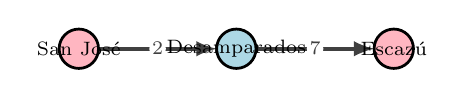
\begin{tikzpicture}
 \Vertex[x=0, y=0, color=LightPink, size=0.5, label={San José}]{A}
 \Vertex[x=2, y=0, color=LightBlue, size=0.5, label={Desamparados}]{C}
 \Edge[label=$2$, Direct](A)(C)
 \Vertex[x=4, y=0, color=LightPink, size=0.5, label={Escazú}]{B}
 \Edge[label=$7$, Direct](C)(B)
\end{tikzpicture}
\end{center}
\begin{center}

\begin{tikzpicture}
 \Vertex[x=0, y=0, color=LightPink, size=0.5, label={San José}]{A}
 \Vertex[x=2, y=0, color=LightPink, size=0.5, label={Desamparados}]{C}
 \Edge[label=$2$, Direct](A)(C)
\end{tikzpicture}
\end{center}
\begin{center}
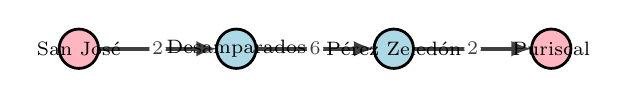
\begin{tikzpicture}
 \Vertex[x=0, y=0, color=LightPink, size=0.5, label={San José}]{A}
 \Vertex[x=2, y=0, color=LightBlue, size=0.5, label={Desamparados}]{C}
 \Edge[label=$2$, Direct](A)(C)
 \Vertex[x=4, y=0, color=LightBlue, size=0.5, label={Pérez Zeledón}]{I}
 \Edge[label=$6$, Direct](C)(I)
 \Vertex[x=6, y=0, color=LightPink, size=0.5, label={Puriscal}]{D}
 \Edge[label=$2$, Direct](I)(D)
\end{tikzpicture}
\end{center}
\begin{center}
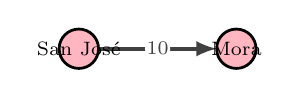
\begin{tikzpicture}
 \Vertex[x=0, y=0, color=LightPink, size=0.5, label={San José}]{A}
 \Vertex[x=2, y=0, color=LightPink, size=0.5, label={Mora}]{E}
 \Edge[label=$10$, Direct](A)(E)
\end{tikzpicture}
\end{center}
\begin{center}
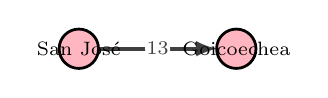
\begin{tikzpicture}
 \Vertex[x=0, y=0, color=LightPink, size=0.5, label={San José}]{A}
 \Vertex[x=2, y=0, color=LightPink, size=0.5, label={Goicoechea}]{F}
 \Edge[label=$13$, Direct](A)(F)
\end{tikzpicture}
\end{center}
\begin{center}
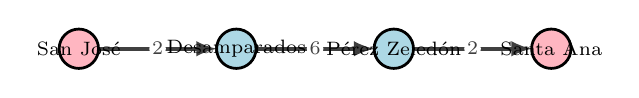
\begin{tikzpicture}
 \Vertex[x=0, y=0, color=LightPink, size=0.5, label={San José}]{A}
 \Vertex[x=2, y=0, color=LightBlue, size=0.5, label={Desamparados}]{C}
 \Edge[label=$2$, Direct](A)(C)
 \Vertex[x=4, y=0, color=LightBlue, size=0.5, label={Pérez Zeledón}]{I}
 \Edge[label=$6$, Direct](C)(I)
 \Vertex[x=6, y=0, color=LightPink, size=0.5, label={Santa Ana}]{G}
 \Edge[label=$2$, Direct](I)(G)
\end{tikzpicture}
\end{center}
\begin{center}

\begin{tikzpicture}
 \Vertex[x=0, y=0, color=LightPink, size=0.5, label={San José}]{A}
 \Vertex[x=2, y=0, color=LightBlue, size=0.5, label={Desamparados}]{C}
 \Edge[label=$2$, Direct](A)(C)
 \Vertex[x=4, y=0, color=LightBlue, size=0.5, label={Pérez Zeledón}]{I}
 \Edge[label=$6$, Direct](C)(I)
 \Vertex[x=6, y=0, color=LightPink, size=0.5, label={Alajuelita}]{H}
 \Edge[label=$2$, Direct](I)(H)
\end{tikzpicture}
\end{center}
\begin{center}
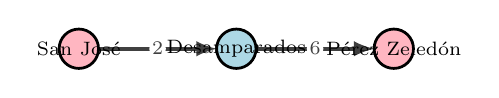
\begin{tikzpicture}
 \Vertex[x=0, y=0, color=LightPink, size=0.5, label={San José}]{A}
 \Vertex[x=2, y=0, color=LightBlue, size=0.5, label={Desamparados}]{C}
 \Edge[label=$2$, Direct](A)(C)
 \Vertex[x=4, y=0, color=LightPink, size=0.5, label={Pérez Zeledón}]{I}
 \Edge[label=$6$, Direct](C)(I)
\end{tikzpicture}
\end{center}
\begin{center}

\begin{tikzpicture}
 \Vertex[x=0, y=0, color=LightPink, size=0.5, label={San José}]{A}
 \Vertex[x=2, y=0, color=LightBlue, size=0.5, label={Desamparados}]{C}
 \Edge[label=$2$, Direct](A)(C)
 \Vertex[x=4, y=0, color=LightPink, size=0.5, label={Curridabat}]{J}
 \Edge[label=$5$, Direct](C)(J)
\end{tikzpicture}
\end{center}
\section*{Current city: Escazú}
\begin{center}
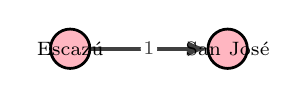
\begin{tikzpicture}
 \Vertex[x=0, y=0, color=LightPink, size=0.5, label={Escazú}]{B}
 \Vertex[x=2, y=0, color=LightPink, size=0.5, label={San José}]{A}
 \Edge[label=$1$, Direct](B)(A)
\end{tikzpicture}
\end{center}
\begin{center}
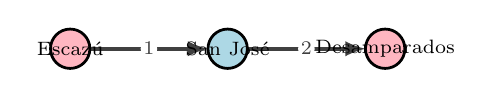
\begin{tikzpicture}
 \Vertex[x=0, y=0, color=LightPink, size=0.5, label={Escazú}]{B}
 \Vertex[x=2, y=0, color=LightBlue, size=0.5, label={San José}]{A}
 \Edge[label=$1$, Direct](B)(A)
 \Vertex[x=4, y=0, color=LightPink, size=0.5, label={Desamparados}]{C}
 \Edge[label=$2$, Direct](A)(C)
\end{tikzpicture}
\end{center}
\begin{center}
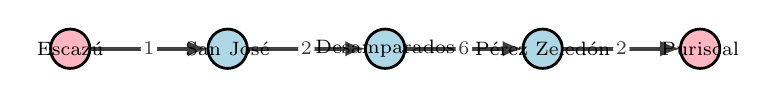
\begin{tikzpicture}
 \Vertex[x=0, y=0, color=LightPink, size=0.5, label={Escazú}]{B}
 \Vertex[x=2, y=0, color=LightBlue, size=0.5, label={San José}]{A}
 \Edge[label=$1$, Direct](B)(A)
 \Vertex[x=4, y=0, color=LightBlue, size=0.5, label={Desamparados}]{C}
 \Edge[label=$2$, Direct](A)(C)
 \Vertex[x=6, y=0, color=LightBlue, size=0.5, label={Pérez Zeledón}]{I}
 \Edge[label=$6$, Direct](C)(I)
 \Vertex[x=8, y=0, color=LightPink, size=0.5, label={Puriscal}]{D}
 \Edge[label=$2$, Direct](I)(D)
\end{tikzpicture}
\end{center}
\begin{center}
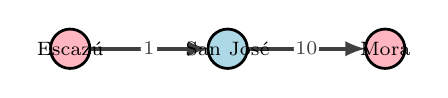
\begin{tikzpicture}
 \Vertex[x=0, y=0, color=LightPink, size=0.5, label={Escazú}]{B}
 \Vertex[x=2, y=0, color=LightBlue, size=0.5, label={San José}]{A}
 \Edge[label=$1$, Direct](B)(A)
 \Vertex[x=4, y=0, color=LightPink, size=0.5, label={Mora}]{E}
 \Edge[label=$10$, Direct](A)(E)
\end{tikzpicture}
\end{center}
\begin{center}
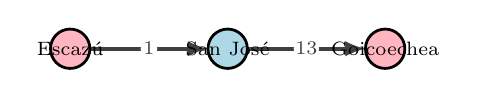
\begin{tikzpicture}
 \Vertex[x=0, y=0, color=LightPink, size=0.5, label={Escazú}]{B}
 \Vertex[x=2, y=0, color=LightBlue, size=0.5, label={San José}]{A}
 \Edge[label=$1$, Direct](B)(A)
 \Vertex[x=4, y=0, color=LightPink, size=0.5, label={Goicoechea}]{F}
 \Edge[label=$13$, Direct](A)(F)
\end{tikzpicture}
\end{center}
\begin{center}
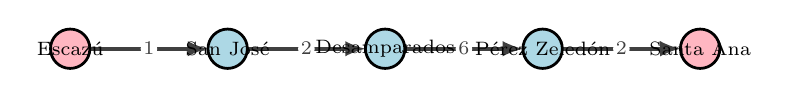
\begin{tikzpicture}
 \Vertex[x=0, y=0, color=LightPink, size=0.5, label={Escazú}]{B}
 \Vertex[x=2, y=0, color=LightBlue, size=0.5, label={San José}]{A}
 \Edge[label=$1$, Direct](B)(A)
 \Vertex[x=4, y=0, color=LightBlue, size=0.5, label={Desamparados}]{C}
 \Edge[label=$2$, Direct](A)(C)
 \Vertex[x=6, y=0, color=LightBlue, size=0.5, label={Pérez Zeledón}]{I}
 \Edge[label=$6$, Direct](C)(I)
 \Vertex[x=8, y=0, color=LightPink, size=0.5, label={Santa Ana}]{G}
 \Edge[label=$2$, Direct](I)(G)
\end{tikzpicture}
\end{center}
\begin{center}
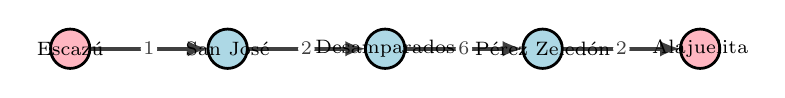
\begin{tikzpicture}
 \Vertex[x=0, y=0, color=LightPink, size=0.5, label={Escazú}]{B}
 \Vertex[x=2, y=0, color=LightBlue, size=0.5, label={San José}]{A}
 \Edge[label=$1$, Direct](B)(A)
 \Vertex[x=4, y=0, color=LightBlue, size=0.5, label={Desamparados}]{C}
 \Edge[label=$2$, Direct](A)(C)
 \Vertex[x=6, y=0, color=LightBlue, size=0.5, label={Pérez Zeledón}]{I}
 \Edge[label=$6$, Direct](C)(I)
 \Vertex[x=8, y=0, color=LightPink, size=0.5, label={Alajuelita}]{H}
 \Edge[label=$2$, Direct](I)(H)
\end{tikzpicture}
\end{center}
\begin{center}
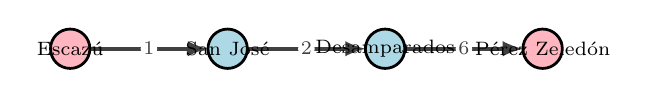
\begin{tikzpicture}
 \Vertex[x=0, y=0, color=LightPink, size=0.5, label={Escazú}]{B}
 \Vertex[x=2, y=0, color=LightBlue, size=0.5, label={San José}]{A}
 \Edge[label=$1$, Direct](B)(A)
 \Vertex[x=4, y=0, color=LightBlue, size=0.5, label={Desamparados}]{C}
 \Edge[label=$2$, Direct](A)(C)
 \Vertex[x=6, y=0, color=LightPink, size=0.5, label={Pérez Zeledón}]{I}
 \Edge[label=$6$, Direct](C)(I)
\end{tikzpicture}
\end{center}
\begin{center}
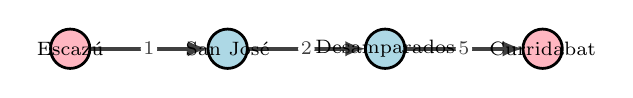
\begin{tikzpicture}
 \Vertex[x=0, y=0, color=LightPink, size=0.5, label={Escazú}]{B}
 \Vertex[x=2, y=0, color=LightBlue, size=0.5, label={San José}]{A}
 \Edge[label=$1$, Direct](B)(A)
 \Vertex[x=4, y=0, color=LightBlue, size=0.5, label={Desamparados}]{C}
 \Edge[label=$2$, Direct](A)(C)
 \Vertex[x=6, y=0, color=LightPink, size=0.5, label={Curridabat}]{J}
 \Edge[label=$5$, Direct](C)(J)
\end{tikzpicture}
\end{center}
\section*{Current city: Desamparados}
\begin{center}
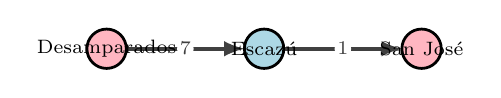
\begin{tikzpicture}
 \Vertex[x=0, y=0, color=LightPink, size=0.5, label={Desamparados}]{C}
 \Vertex[x=2, y=0, color=LightBlue, size=0.5, label={Escazú}]{B}
 \Edge[label=$7$, Direct](C)(B)
 \Vertex[x=4, y=0, color=LightPink, size=0.5, label={San José}]{A}
 \Edge[label=$1$, Direct](B)(A)
\end{tikzpicture}
\end{center}
\begin{center}
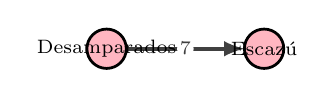
\begin{tikzpicture}
 \Vertex[x=0, y=0, color=LightPink, size=0.5, label={Desamparados}]{C}
 \Vertex[x=2, y=0, color=LightPink, size=0.5, label={Escazú}]{B}
 \Edge[label=$7$, Direct](C)(B)
\end{tikzpicture}
\end{center}
\begin{center}
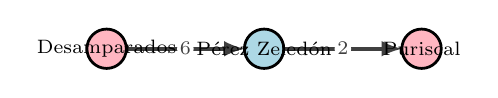
\begin{tikzpicture}
 \Vertex[x=0, y=0, color=LightPink, size=0.5, label={Desamparados}]{C}
 \Vertex[x=2, y=0, color=LightBlue, size=0.5, label={Pérez Zeledón}]{I}
 \Edge[label=$6$, Direct](C)(I)
 \Vertex[x=4, y=0, color=LightPink, size=0.5, label={Puriscal}]{D}
 \Edge[label=$2$, Direct](I)(D)
\end{tikzpicture}
\end{center}
\begin{center}
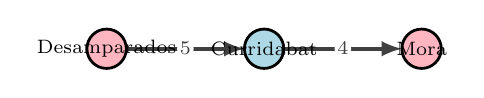
\begin{tikzpicture}
 \Vertex[x=0, y=0, color=LightPink, size=0.5, label={Desamparados}]{C}
 \Vertex[x=2, y=0, color=LightBlue, size=0.5, label={Curridabat}]{J}
 \Edge[label=$5$, Direct](C)(J)
 \Vertex[x=4, y=0, color=LightPink, size=0.5, label={Mora}]{E}
 \Edge[label=$4$, Direct](J)(E)
\end{tikzpicture}
\end{center}
\begin{center}
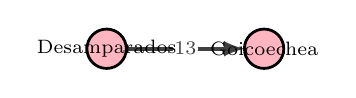
\begin{tikzpicture}
 \Vertex[x=0, y=0, color=LightPink, size=0.5, label={Desamparados}]{C}
 \Vertex[x=2, y=0, color=LightPink, size=0.5, label={Goicoechea}]{F}
 \Edge[label=$13$, Direct](C)(F)
\end{tikzpicture}
\end{center}
\begin{center}
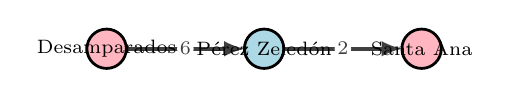
\begin{tikzpicture}
 \Vertex[x=0, y=0, color=LightPink, size=0.5, label={Desamparados}]{C}
 \Vertex[x=2, y=0, color=LightBlue, size=0.5, label={Pérez Zeledón}]{I}
 \Edge[label=$6$, Direct](C)(I)
 \Vertex[x=4, y=0, color=LightPink, size=0.5, label={Santa Ana}]{G}
 \Edge[label=$2$, Direct](I)(G)
\end{tikzpicture}
\end{center}
\begin{center}

\begin{tikzpicture}
 \Vertex[x=0, y=0, color=LightPink, size=0.5, label={Desamparados}]{C}
 \Vertex[x=2, y=0, color=LightBlue, size=0.5, label={Pérez Zeledón}]{I}
 \Edge[label=$6$, Direct](C)(I)
 \Vertex[x=4, y=0, color=LightPink, size=0.5, label={Alajuelita}]{H}
 \Edge[label=$2$, Direct](I)(H)
\end{tikzpicture}
\end{center}
\begin{center}
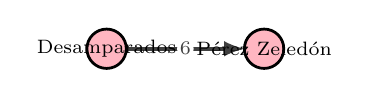
\begin{tikzpicture}
 \Vertex[x=0, y=0, color=LightPink, size=0.5, label={Desamparados}]{C}
 \Vertex[x=2, y=0, color=LightPink, size=0.5, label={Pérez Zeledón}]{I}
 \Edge[label=$6$, Direct](C)(I)
\end{tikzpicture}
\end{center}
\begin{center}

\begin{tikzpicture}
 \Vertex[x=0, y=0, color=LightPink, size=0.5, label={Desamparados}]{C}
 \Vertex[x=2, y=0, color=LightPink, size=0.5, label={Curridabat}]{J}
 \Edge[label=$5$, Direct](C)(J)
\end{tikzpicture}
\end{center}
\section*{Current city: Puriscal}
\begin{center}
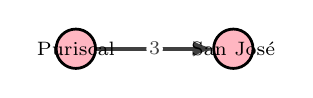
\begin{tikzpicture}
 \Vertex[x=0, y=0, color=LightPink, size=0.5, label={Puriscal}]{D}
 \Vertex[x=2, y=0, color=LightPink, size=0.5, label={San José}]{A}
 \Edge[label=$3$, Direct](D)(A)
\end{tikzpicture}
\end{center}
\begin{center}
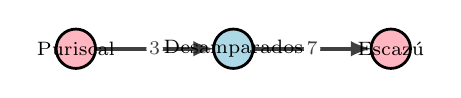
\begin{tikzpicture}
 \Vertex[x=0, y=0, color=LightPink, size=0.5, label={Puriscal}]{D}
 \Vertex[x=2, y=0, color=LightBlue, size=0.5, label={Desamparados}]{C}
 \Edge[label=$3$, Direct](D)(C)
 \Vertex[x=4, y=0, color=LightPink, size=0.5, label={Escazú}]{B}
 \Edge[label=$7$, Direct](C)(B)
\end{tikzpicture}
\end{center}
\begin{center}
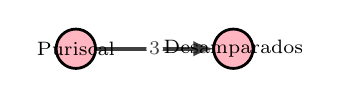
\begin{tikzpicture}
 \Vertex[x=0, y=0, color=LightPink, size=0.5, label={Puriscal}]{D}
 \Vertex[x=2, y=0, color=LightPink, size=0.5, label={Desamparados}]{C}
 \Edge[label=$3$, Direct](D)(C)
\end{tikzpicture}
\end{center}
\begin{center}
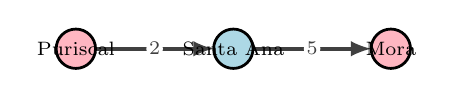
\begin{tikzpicture}
 \Vertex[x=0, y=0, color=LightPink, size=0.5, label={Puriscal}]{D}
 \Vertex[x=2, y=0, color=LightBlue, size=0.5, label={Santa Ana}]{G}
 \Edge[label=$2$, Direct](D)(G)
 \Vertex[x=4, y=0, color=LightPink, size=0.5, label={Mora}]{E}
 \Edge[label=$5$, Direct](G)(E)
\end{tikzpicture}
\end{center}
\begin{center}
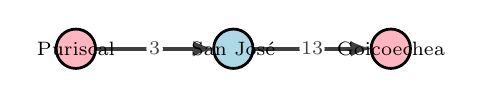
\begin{tikzpicture}
 \Vertex[x=0, y=0, color=LightPink, size=0.5, label={Puriscal}]{D}
 \Vertex[x=2, y=0, color=LightBlue, size=0.5, label={San José}]{A}
 \Edge[label=$3$, Direct](D)(A)
 \Vertex[x=4, y=0, color=LightPink, size=0.5, label={Goicoechea}]{F}
 \Edge[label=$13$, Direct](A)(F)
\end{tikzpicture}
\end{center}
\begin{center}
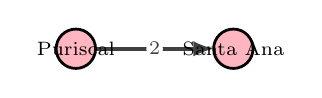
\begin{tikzpicture}
 \Vertex[x=0, y=0, color=LightPink, size=0.5, label={Puriscal}]{D}
 \Vertex[x=2, y=0, color=LightPink, size=0.5, label={Santa Ana}]{G}
 \Edge[label=$2$, Direct](D)(G)
\end{tikzpicture}
\end{center}
\begin{center}
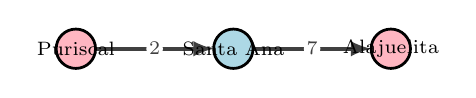
\begin{tikzpicture}
 \Vertex[x=0, y=0, color=LightPink, size=0.5, label={Puriscal}]{D}
 \Vertex[x=2, y=0, color=LightBlue, size=0.5, label={Santa Ana}]{G}
 \Edge[label=$2$, Direct](D)(G)
 \Vertex[x=4, y=0, color=LightPink, size=0.5, label={Alajuelita}]{H}
 \Edge[label=$7$, Direct](G)(H)
\end{tikzpicture}
\end{center}
\begin{center}
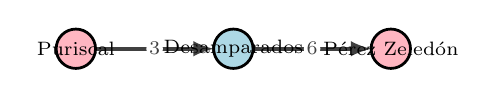
\begin{tikzpicture}
 \Vertex[x=0, y=0, color=LightPink, size=0.5, label={Puriscal}]{D}
 \Vertex[x=2, y=0, color=LightBlue, size=0.5, label={Desamparados}]{C}
 \Edge[label=$3$, Direct](D)(C)
 \Vertex[x=4, y=0, color=LightPink, size=0.5, label={Pérez Zeledón}]{I}
 \Edge[label=$6$, Direct](C)(I)
\end{tikzpicture}
\end{center}
\begin{center}
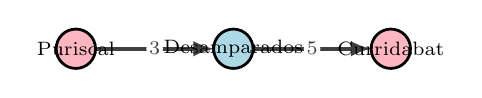
\begin{tikzpicture}
 \Vertex[x=0, y=0, color=LightPink, size=0.5, label={Puriscal}]{D}
 \Vertex[x=2, y=0, color=LightBlue, size=0.5, label={Desamparados}]{C}
 \Edge[label=$3$, Direct](D)(C)
 \Vertex[x=4, y=0, color=LightPink, size=0.5, label={Curridabat}]{J}
 \Edge[label=$5$, Direct](C)(J)
\end{tikzpicture}
\end{center}
\section*{Current city: Mora}
\begin{center}
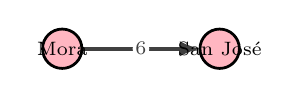
\begin{tikzpicture}
 \Vertex[x=0, y=0, color=LightPink, size=0.5, label={Mora}]{E}
 \Vertex[x=2, y=0, color=LightPink, size=0.5, label={San José}]{A}
 \Edge[label=$6$, Direct](E)(A)
\end{tikzpicture}
\end{center}
\begin{center}
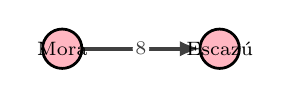
\begin{tikzpicture}
 \Vertex[x=0, y=0, color=LightPink, size=0.5, label={Mora}]{E}
 \Vertex[x=2, y=0, color=LightPink, size=0.5, label={Escazú}]{B}
 \Edge[label=$8$, Direct](E)(B)
\end{tikzpicture}
\end{center}
\begin{center}
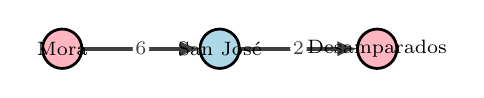
\begin{tikzpicture}
 \Vertex[x=0, y=0, color=LightPink, size=0.5, label={Mora}]{E}
 \Vertex[x=2, y=0, color=LightBlue, size=0.5, label={San José}]{A}
 \Edge[label=$6$, Direct](E)(A)
 \Vertex[x=4, y=0, color=LightPink, size=0.5, label={Desamparados}]{C}
 \Edge[label=$2$, Direct](A)(C)
\end{tikzpicture}
\end{center}
\begin{center}
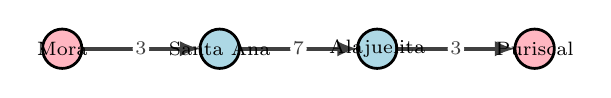
\begin{tikzpicture}
 \Vertex[x=0, y=0, color=LightPink, size=0.5, label={Mora}]{E}
 \Vertex[x=2, y=0, color=LightBlue, size=0.5, label={Santa Ana}]{G}
 \Edge[label=$3$, Direct](E)(G)
 \Vertex[x=4, y=0, color=LightBlue, size=0.5, label={Alajuelita}]{H}
 \Edge[label=$7$, Direct](G)(H)
 \Vertex[x=6, y=0, color=LightPink, size=0.5, label={Puriscal}]{D}
 \Edge[label=$3$, Direct](H)(D)
\end{tikzpicture}
\end{center}
\begin{center}
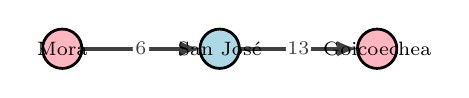
\begin{tikzpicture}
 \Vertex[x=0, y=0, color=LightPink, size=0.5, label={Mora}]{E}
 \Vertex[x=2, y=0, color=LightBlue, size=0.5, label={San José}]{A}
 \Edge[label=$6$, Direct](E)(A)
 \Vertex[x=4, y=0, color=LightPink, size=0.5, label={Goicoechea}]{F}
 \Edge[label=$13$, Direct](A)(F)
\end{tikzpicture}
\end{center}
\begin{center}
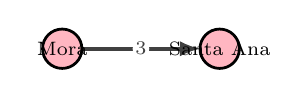
\begin{tikzpicture}
 \Vertex[x=0, y=0, color=LightPink, size=0.5, label={Mora}]{E}
 \Vertex[x=2, y=0, color=LightPink, size=0.5, label={Santa Ana}]{G}
 \Edge[label=$3$, Direct](E)(G)
\end{tikzpicture}
\end{center}
\begin{center}
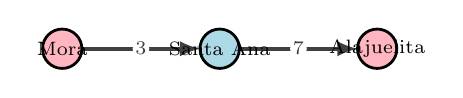
\begin{tikzpicture}
 \Vertex[x=0, y=0, color=LightPink, size=0.5, label={Mora}]{E}
 \Vertex[x=2, y=0, color=LightBlue, size=0.5, label={Santa Ana}]{G}
 \Edge[label=$3$, Direct](E)(G)
 \Vertex[x=4, y=0, color=LightPink, size=0.5, label={Alajuelita}]{H}
 \Edge[label=$7$, Direct](G)(H)
\end{tikzpicture}
\end{center}
\begin{center}
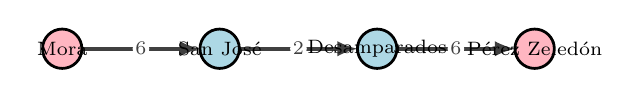
\begin{tikzpicture}
 \Vertex[x=0, y=0, color=LightPink, size=0.5, label={Mora}]{E}
 \Vertex[x=2, y=0, color=LightBlue, size=0.5, label={San José}]{A}
 \Edge[label=$6$, Direct](E)(A)
 \Vertex[x=4, y=0, color=LightBlue, size=0.5, label={Desamparados}]{C}
 \Edge[label=$2$, Direct](A)(C)
 \Vertex[x=6, y=0, color=LightPink, size=0.5, label={Pérez Zeledón}]{I}
 \Edge[label=$6$, Direct](C)(I)
\end{tikzpicture}
\end{center}
\begin{center}
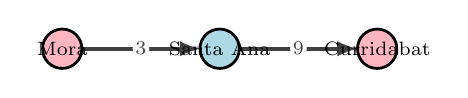
\begin{tikzpicture}
 \Vertex[x=0, y=0, color=LightPink, size=0.5, label={Mora}]{E}
 \Vertex[x=2, y=0, color=LightBlue, size=0.5, label={Santa Ana}]{G}
 \Edge[label=$3$, Direct](E)(G)
 \Vertex[x=4, y=0, color=LightPink, size=0.5, label={Curridabat}]{J}
 \Edge[label=$9$, Direct](G)(J)
\end{tikzpicture}
\end{center}
\section*{Current city: Goicoechea}
\begin{center}
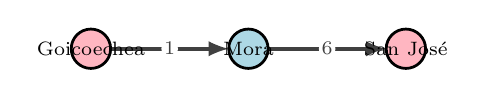
\begin{tikzpicture}
 \Vertex[x=0, y=0, color=LightPink, size=0.5, label={Goicoechea}]{F}
 \Vertex[x=2, y=0, color=LightBlue, size=0.5, label={Mora}]{E}
 \Edge[label=$1$, Direct](F)(E)
 \Vertex[x=4, y=0, color=LightPink, size=0.5, label={San José}]{A}
 \Edge[label=$6$, Direct](E)(A)
\end{tikzpicture}
\end{center}
\begin{center}
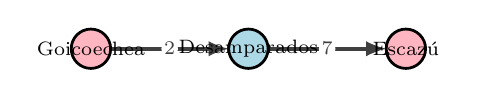
\begin{tikzpicture}
 \Vertex[x=0, y=0, color=LightPink, size=0.5, label={Goicoechea}]{F}
 \Vertex[x=2, y=0, color=LightBlue, size=0.5, label={Desamparados}]{C}
 \Edge[label=$2$, Direct](F)(C)
 \Vertex[x=4, y=0, color=LightPink, size=0.5, label={Escazú}]{B}
 \Edge[label=$7$, Direct](C)(B)
\end{tikzpicture}
\end{center}
\begin{center}

\begin{tikzpicture}
 \Vertex[x=0, y=0, color=LightPink, size=0.5, label={Goicoechea}]{F}
 \Vertex[x=2, y=0, color=LightPink, size=0.5, label={Desamparados}]{C}
 \Edge[label=$2$, Direct](F)(C)
\end{tikzpicture}
\end{center}
\begin{center}

\begin{tikzpicture}
 \Vertex[x=0, y=0, color=LightPink, size=0.5, label={Goicoechea}]{F}
 \Vertex[x=2, y=0, color=LightBlue, size=0.5, label={Desamparados}]{C}
 \Edge[label=$2$, Direct](F)(C)
 \Vertex[x=4, y=0, color=LightBlue, size=0.5, label={Pérez Zeledón}]{I}
 \Edge[label=$6$, Direct](C)(I)
 \Vertex[x=6, y=0, color=LightPink, size=0.5, label={Puriscal}]{D}
 \Edge[label=$2$, Direct](I)(D)
\end{tikzpicture}
\end{center}
\begin{center}
\begin{tikzpicture}
 \Vertex[x=0, y=0, color=LightPink, size=0.5, label={Goicoechea}]{F}
 \Vertex[x=2, y=0, color=LightPink, size=0.5, label={Mora}]{E}
 \Edge[label=$1$, Direct](F)(E)
\end{tikzpicture}
\end{center}
\begin{center}
\begin{tikzpicture}
 \Vertex[x=0, y=0, color=LightPink, size=0.5, label={Goicoechea}]{F}
 \Vertex[x=2, y=0, color=LightBlue, size=0.5, label={Mora}]{E}
 \Edge[label=$1$, Direct](F)(E)
 \Vertex[x=4, y=0, color=LightPink, size=0.5, label={Santa Ana}]{G}
 \Edge[label=$3$, Direct](E)(G)
\end{tikzpicture}
\end{center}
\begin{center}
\begin{tikzpicture}
 \Vertex[x=0, y=0, color=LightPink, size=0.5, label={Goicoechea}]{F}
 \Vertex[x=2, y=0, color=LightBlue, size=0.5, label={Desamparados}]{C}
 \Edge[label=$2$, Direct](F)(C)
 \Vertex[x=4, y=0, color=LightBlue, size=0.5, label={Pérez Zeledón}]{I}
 \Edge[label=$6$, Direct](C)(I)
 \Vertex[x=6, y=0, color=LightPink, size=0.5, label={Alajuelita}]{H}
 \Edge[label=$2$, Direct](I)(H)
\end{tikzpicture}
\end{center}
\begin{center}
\begin{tikzpicture}
 \Vertex[x=0, y=0, color=LightPink, size=0.5, label={Goicoechea}]{F}
 \Vertex[x=2, y=0, color=LightBlue, size=0.5, label={Desamparados}]{C}
 \Edge[label=$2$, Direct](F)(C)
 \Vertex[x=4, y=0, color=LightPink, size=0.5, label={Pérez Zeledón}]{I}
 \Edge[label=$6$, Direct](C)(I)
\end{tikzpicture}
\end{center}
\begin{center}
\begin{tikzpicture}
 \Vertex[x=0, y=0, color=LightPink, size=0.5, label={Goicoechea}]{F}
 \Vertex[x=2, y=0, color=LightBlue, size=0.5, label={Desamparados}]{C}
 \Edge[label=$2$, Direct](F)(C)
 \Vertex[x=4, y=0, color=LightPink, size=0.5, label={Curridabat}]{J}
 \Edge[label=$5$, Direct](C)(J)
\end{tikzpicture}
\end{center}
\section*{Current city: Santa Ana}
\begin{center}
\begin{tikzpicture}
 \Vertex[x=0, y=0, color=LightPink, size=0.5, label={Santa Ana}]{G}
 \Vertex[x=2, y=0, color=LightPink, size=0.5, label={San José}]{A}
 \Edge[label=$9$, Direct](G)(A)
\end{tikzpicture}
\end{center}
\begin{center}
\begin{tikzpicture}
 \Vertex[x=0, y=0, color=LightPink, size=0.5, label={Santa Ana}]{G}
 \Vertex[x=2, y=0, color=LightBlue, size=0.5, label={Alajuelita}]{H}
 \Edge[label=$7$, Direct](G)(H)
 \Vertex[x=4, y=0, color=LightPink, size=0.5, label={Escazú}]{B}
 \Edge[label=$1$, Direct](H)(B)
\end{tikzpicture}
\end{center}
\begin{center}
\begin{tikzpicture}
 \Vertex[x=0, y=0, color=LightPink, size=0.5, label={Santa Ana}]{G}
 \Vertex[x=2, y=0, color=LightBlue, size=0.5, label={San José}]{A}
 \Edge[label=$9$, Direct](G)(A)
 \Vertex[x=4, y=0, color=LightPink, size=0.5, label={Desamparados}]{C}
 \Edge[label=$2$, Direct](A)(C)
\end{tikzpicture}
\end{center}
\begin{center}
\begin{tikzpicture}
 \Vertex[x=0, y=0, color=LightPink, size=0.5, label={Santa Ana}]{G}
 \Vertex[x=2, y=0, color=LightBlue, size=0.5, label={Alajuelita}]{H}
 \Edge[label=$7$, Direct](G)(H)
 \Vertex[x=4, y=0, color=LightPink, size=0.5, label={Puriscal}]{D}
 \Edge[label=$3$, Direct](H)(D)
\end{tikzpicture}
\end{center}
\begin{center}
\begin{tikzpicture}
 \Vertex[x=0, y=0, color=LightPink, size=0.5, label={Santa Ana}]{G}
 \Vertex[x=2, y=0, color=LightPink, size=0.5, label={Mora}]{E}
 \Edge[label=$5$, Direct](G)(E)
\end{tikzpicture}
\end{center}
\begin{center}
\begin{tikzpicture}
 \Vertex[x=0, y=0, color=LightPink, size=0.5, label={Santa Ana}]{G}
 \Vertex[x=2, y=0, color=LightBlue, size=0.5, label={Curridabat}]{J}
 \Edge[label=$9$, Direct](G)(J)
 \Vertex[x=4, y=0, color=LightPink, size=0.5, label={Goicoechea}]{F}
 \Edge[label=$9$, Direct](J)(F)
\end{tikzpicture}
\end{center}
\begin{center}
\begin{tikzpicture}
 \Vertex[x=0, y=0, color=LightPink, size=0.5, label={Santa Ana}]{G}
 \Vertex[x=2, y=0, color=LightPink, size=0.5, label={Alajuelita}]{H}
 \Edge[label=$7$, Direct](G)(H)
\end{tikzpicture}
\end{center}
\begin{center}
\begin{tikzpicture}
 \Vertex[x=0, y=0, color=LightPink, size=0.5, label={Santa Ana}]{G}
 \Vertex[x=2, y=0, color=LightBlue, size=0.5, label={San José}]{A}
 \Edge[label=$9$, Direct](G)(A)
 \Vertex[x=4, y=0, color=LightBlue, size=0.5, label={Desamparados}]{C}
 \Edge[label=$2$, Direct](A)(C)
 \Vertex[x=6, y=0, color=LightPink, size=0.5, label={Pérez Zeledón}]{I}
 \Edge[label=$6$, Direct](C)(I)
\end{tikzpicture}
\end{center}
\begin{center}
\begin{tikzpicture}
 \Vertex[x=0, y=0, color=LightPink, size=0.5, label={Santa Ana}]{G}
 \Vertex[x=2, y=0, color=LightPink, size=0.5, label={Curridabat}]{J}
 \Edge[label=$9$, Direct](G)(J)
\end{tikzpicture}
\end{center}
\section*{Current city: Alajuelita}
\begin{center}
\begin{tikzpicture}
 \Vertex[x=0, y=0, color=LightPink, size=0.5, label={Alajuelita}]{H}
 \Vertex[x=2, y=0, color=LightBlue, size=0.5, label={Escazú}]{B}
 \Edge[label=$1$, Direct](H)(B)
 \Vertex[x=4, y=0, color=LightPink, size=0.5, label={San José}]{A}
 \Edge[label=$1$, Direct](B)(A)
\end{tikzpicture}
\end{center}
\begin{center}
\begin{tikzpicture}
 \Vertex[x=0, y=0, color=LightPink, size=0.5, label={Alajuelita}]{H}
 \Vertex[x=2, y=0, color=LightPink, size=0.5, label={Escazú}]{B}
 \Edge[label=$1$, Direct](H)(B)
\end{tikzpicture}
\end{center}
\begin{center}
\begin{tikzpicture}
 \Vertex[x=0, y=0, color=LightPink, size=0.5, label={Alajuelita}]{H}
 \Vertex[x=2, y=0, color=LightBlue, size=0.5, label={Escazú}]{B}
 \Edge[label=$1$, Direct](H)(B)
 \Vertex[x=4, y=0, color=LightBlue, size=0.5, label={San José}]{A}
 \Edge[label=$1$, Direct](B)(A)
 \Vertex[x=6, y=0, color=LightPink, size=0.5, label={Desamparados}]{C}
 \Edge[label=$2$, Direct](A)(C)
\end{tikzpicture}
\end{center}
\begin{center}
\begin{tikzpicture}
 \Vertex[x=0, y=0, color=LightPink, size=0.5, label={Alajuelita}]{H}
 \Vertex[x=2, y=0, color=LightPink, size=0.5, label={Puriscal}]{D}
 \Edge[label=$3$, Direct](H)(D)
\end{tikzpicture}
\end{center}
\begin{center}
\begin{tikzpicture}
 \Vertex[x=0, y=0, color=LightPink, size=0.5, label={Alajuelita}]{H}
 \Vertex[x=2, y=0, color=LightPink, size=0.5, label={Mora}]{E}
 \Edge[label=$8$, Direct](H)(E)
\end{tikzpicture}
\end{center}
\begin{center}
\begin{tikzpicture}
 \Vertex[x=0, y=0, color=LightPink, size=0.5, label={Alajuelita}]{H}
 \Vertex[x=2, y=0, color=LightBlue, size=0.5, label={Escazú}]{B}
 \Edge[label=$1$, Direct](H)(B)
 \Vertex[x=4, y=0, color=LightBlue, size=0.5, label={San José}]{A}
 \Edge[label=$1$, Direct](B)(A)
 \Vertex[x=6, y=0, color=LightPink, size=0.5, label={Goicoechea}]{F}
 \Edge[label=$13$, Direct](A)(F)
\end{tikzpicture}
\end{center}
\begin{center}
\begin{tikzpicture}
 \Vertex[x=0, y=0, color=LightPink, size=0.5, label={Alajuelita}]{H}
 \Vertex[x=2, y=0, color=LightBlue, size=0.5, label={Puriscal}]{D}
 \Edge[label=$3$, Direct](H)(D)
 \Vertex[x=4, y=0, color=LightPink, size=0.5, label={Santa Ana}]{G}
 \Edge[label=$2$, Direct](D)(G)
\end{tikzpicture}
\end{center}
\begin{center}
\begin{tikzpicture}
 \Vertex[x=0, y=0, color=LightPink, size=0.5, label={Alajuelita}]{H}
 \Vertex[x=2, y=0, color=LightBlue, size=0.5, label={Escazú}]{B}
 \Edge[label=$1$, Direct](H)(B)
 \Vertex[x=4, y=0, color=LightBlue, size=0.5, label={San José}]{A}
 \Edge[label=$1$, Direct](B)(A)
 \Vertex[x=6, y=0, color=LightBlue, size=0.5, label={Desamparados}]{C}
 \Edge[label=$2$, Direct](A)(C)
 \Vertex[x=8, y=0, color=LightPink, size=0.5, label={Pérez Zeledón}]{I}
 \Edge[label=$6$, Direct](C)(I)
\end{tikzpicture}
\end{center}
\begin{center}
\begin{tikzpicture}
 \Vertex[x=0, y=0, color=LightPink, size=0.5, label={Alajuelita}]{H}
 \Vertex[x=2, y=0, color=LightBlue, size=0.5, label={Escazú}]{B}
 \Edge[label=$1$, Direct](H)(B)
 \Vertex[x=4, y=0, color=LightBlue, size=0.5, label={San José}]{A}
 \Edge[label=$1$, Direct](B)(A)
 \Vertex[x=6, y=0, color=LightBlue, size=0.5, label={Desamparados}]{C}
 \Edge[label=$2$, Direct](A)(C)
 \Vertex[x=8, y=0, color=LightPink, size=0.5, label={Curridabat}]{J}
 \Edge[label=$5$, Direct](C)(J)
\end{tikzpicture}
\end{center}
\section*{Current city: Pérez Zeledón}
\begin{center}
\begin{tikzpicture}
 \Vertex[x=0, y=0, color=LightPink, size=0.5, label={Pérez Zeledón}]{I}
 \Vertex[x=2, y=0, color=LightPink, size=0.5, label={San José}]{A}
 \Edge[label=$2$, Direct](I)(A)
\end{tikzpicture}
\end{center}
\begin{center}
\begin{tikzpicture}
 \Vertex[x=0, y=0, color=LightPink, size=0.5, label={Pérez Zeledón}]{I}
 \Vertex[x=2, y=0, color=LightBlue, size=0.5, label={Alajuelita}]{H}
 \Edge[label=$2$, Direct](I)(H)
 \Vertex[x=4, y=0, color=LightPink, size=0.5, label={Escazú}]{B}
 \Edge[label=$1$, Direct](H)(B)
\end{tikzpicture}
\end{center}
\begin{center}
\begin{tikzpicture}
 \Vertex[x=0, y=0, color=LightPink, size=0.5, label={Pérez Zeledón}]{I}
 \Vertex[x=2, y=0, color=LightBlue, size=0.5, label={San José}]{A}
 \Edge[label=$2$, Direct](I)(A)
 \Vertex[x=4, y=0, color=LightPink, size=0.5, label={Desamparados}]{C}
 \Edge[label=$2$, Direct](A)(C)
\end{tikzpicture}
\end{center}
\begin{center}
\begin{tikzpicture}
 \Vertex[x=0, y=0, color=LightPink, size=0.5, label={Pérez Zeledón}]{I}
 \Vertex[x=2, y=0, color=LightPink, size=0.5, label={Puriscal}]{D}
 \Edge[label=$2$, Direct](I)(D)
\end{tikzpicture}
\end{center}
\begin{center}
\begin{tikzpicture}
 \Vertex[x=0, y=0, color=LightPink, size=0.5, label={Pérez Zeledón}]{I}
 \Vertex[x=2, y=0, color=LightBlue, size=0.5, label={Santa Ana}]{G}
 \Edge[label=$2$, Direct](I)(G)
 \Vertex[x=4, y=0, color=LightPink, size=0.5, label={Mora}]{E}
 \Edge[label=$5$, Direct](G)(E)
\end{tikzpicture}
\end{center}
\begin{center}
\begin{tikzpicture}
 \Vertex[x=0, y=0, color=LightPink, size=0.5, label={Pérez Zeledón}]{I}
 \Vertex[x=2, y=0, color=LightPink, size=0.5, label={Goicoechea}]{F}
 \Edge[label=$7$, Direct](I)(F)
\end{tikzpicture}
\end{center}
\begin{center}
\begin{tikzpicture}
 \Vertex[x=0, y=0, color=LightPink, size=0.5, label={Pérez Zeledón}]{I}
 \Vertex[x=2, y=0, color=LightPink, size=0.5, label={Santa Ana}]{G}
 \Edge[label=$2$, Direct](I)(G)
\end{tikzpicture}
\end{center}
\begin{center}
\begin{tikzpicture}
 \Vertex[x=0, y=0, color=LightPink, size=0.5, label={Pérez Zeledón}]{I}
 \Vertex[x=2, y=0, color=LightPink, size=0.5, label={Alajuelita}]{H}
 \Edge[label=$2$, Direct](I)(H)
\end{tikzpicture}
\end{center}
\begin{center}
\begin{tikzpicture}
 \Vertex[x=0, y=0, color=LightPink, size=0.5, label={Pérez Zeledón}]{I}
 \Vertex[x=2, y=0, color=LightBlue, size=0.5, label={San José}]{A}
 \Edge[label=$2$, Direct](I)(A)
 \Vertex[x=4, y=0, color=LightBlue, size=0.5, label={Desamparados}]{C}
 \Edge[label=$2$, Direct](A)(C)
 \Vertex[x=6, y=0, color=LightPink, size=0.5, label={Curridabat}]{J}
 \Edge[label=$5$, Direct](C)(J)
\end{tikzpicture}
\end{center}
\section*{Current city: Curridabat}
\begin{center}
\begin{tikzpicture}
 \Vertex[x=0, y=0, color=LightPink, size=0.5, label={Curridabat}]{J}
 \Vertex[x=2, y=0, color=LightBlue, size=0.5, label={Escazú}]{B}
 \Edge[label=$3$, Direct](J)(B)
 \Vertex[x=4, y=0, color=LightPink, size=0.5, label={San José}]{A}
 \Edge[label=$1$, Direct](B)(A)
\end{tikzpicture}
\end{center}
\begin{center}
\begin{tikzpicture}
 \Vertex[x=0, y=0, color=LightPink, size=0.5, label={Curridabat}]{J}
 \Vertex[x=2, y=0, color=LightPink, size=0.5, label={Escazú}]{B}
 \Edge[label=$3$, Direct](J)(B)
\end{tikzpicture}
\end{center}
\begin{center}
\begin{tikzpicture}
 \Vertex[x=0, y=0, color=LightPink, size=0.5, label={Curridabat}]{J}
 \Vertex[x=2, y=0, color=LightBlue, size=0.5, label={Escazú}]{B}
 \Edge[label=$3$, Direct](J)(B)
 \Vertex[x=4, y=0, color=LightBlue, size=0.5, label={San José}]{A}
 \Edge[label=$1$, Direct](B)(A)
 \Vertex[x=6, y=0, color=LightPink, size=0.5, label={Desamparados}]{C}
 \Edge[label=$2$, Direct](A)(C)
\end{tikzpicture}
\end{center}
\begin{center}
\begin{tikzpicture}
 \Vertex[x=0, y=0, color=LightPink, size=0.5, label={Curridabat}]{J}
 \Vertex[x=2, y=0, color=LightPink, size=0.5, label={Puriscal}]{D}
 \Edge[label=$9$, Direct](J)(D)
\end{tikzpicture}
\end{center}
\begin{center}
\begin{tikzpicture}
 \Vertex[x=0, y=0, color=LightPink, size=0.5, label={Curridabat}]{J}
 \Vertex[x=2, y=0, color=LightPink, size=0.5, label={Mora}]{E}
 \Edge[label=$4$, Direct](J)(E)
\end{tikzpicture}
\end{center}
\begin{center}
\begin{tikzpicture}
 \Vertex[x=0, y=0, color=LightPink, size=0.5, label={Curridabat}]{J}
 \Vertex[x=2, y=0, color=LightPink, size=0.5, label={Goicoechea}]{F}
 \Edge[label=$9$, Direct](J)(F)
\end{tikzpicture}
\end{center}
\begin{center}
\begin{tikzpicture}
 \Vertex[x=0, y=0, color=LightPink, size=0.5, label={Curridabat}]{J}
 \Vertex[x=2, y=0, color=LightBlue, size=0.5, label={Mora}]{E}
 \Edge[label=$4$, Direct](J)(E)
 \Vertex[x=4, y=0, color=LightPink, size=0.5, label={Santa Ana}]{G}
 \Edge[label=$3$, Direct](E)(G)
\end{tikzpicture}
\end{center}
\begin{center}
\begin{tikzpicture}
 \Vertex[x=0, y=0, color=LightPink, size=0.5, label={Curridabat}]{J}
 \Vertex[x=2, y=0, color=LightPink, size=0.5, label={Alajuelita}]{H}
 \Edge[label=$8$, Direct](J)(H)
\end{tikzpicture}
\end{center}
\begin{center}
\begin{tikzpicture}
 \Vertex[x=0, y=0, color=LightPink, size=0.5, label={Curridabat}]{J}
 \Vertex[x=2, y=0, color=LightPink, size=0.5, label={Pérez Zeledón}]{I}
 \Edge[label=$12$, Direct](J)(I)
\end{tikzpicture}
\end{center}
\end{document}
